\documentclass{article}
\usepackage[utf8]{inputenc}
\usepackage{preamble} % everything is loaded in there, basically.
%\graphicspath{{../figures/}} % set filepath for figures
\usepackage{svg}

%---------------------------------------------------------------------------------------------------------------------------
%% TODO statements
%---------------------------------------------------------------------------------------------------------------------------
\setlength{\marginparwidth}{2.5cm}
\usepackage[colorinlistoftodos]{todonotes}
%\usepackage[disable]{todonotes} % This will disable viewing Todos
\setuptodonotes{size=\scriptsize,backgroundcolor=red!15!white} 

\newcommandx{\colin}[2][1=]{\todo[linecolor=green,backgroundcolor=green!25,bordercolor=green,#1]{\tiny Colin: #2}}

%---------------------------------------------------------------------------------------------------------------------------


%---------------------------------------------------------------------------------------------------------------------------
%% Document Info
%---------------------------------------------------------------------------------------------------------------------------
\title{Topological Electromagnetism of Circuit Components and Measurement Devices}

\author{Colin Roberts}
%---------------------------------------------------------------------------------------------------------------------------



%---------------------------------------------------------------------------------------------------------------------------
%% Document Start
%---------------------------------------------------------------------------------------------------------------------------
\begin{document}

\maketitle

\section*{Comments}
some thoughts in march '22
\begin{itemize}
    \item \url{https://arxiv.org/pdf/1404.1932.pdf}
    \item Topology of waveguides and monogenic fields on spacetime manifolds?
    \item Multipole expansions and monogenics?
    \item Is the Kunneth formula like a generalized way of looking at separation of variables?
    \item \url{https://www.newton.ac.uk/files/seminar/20121025113012301-153414.pdf} seems cool and so does \url{https://wakespace.lib.wfu.edu/bitstream/handle/10339/90751/McConkey_wfu_0248M_11221.pdf}
    \item Sullivan's paper on fluid algebras could be very very interesting. Here is a picture of the idea:
    \begin{figure}[H]
        \centering
        \includegraphics{figures/fluid_algebra.png}
    \end{figure}
    Maybe solenoidal beltrami fields on a compact manifold form a fluid algebra?
\end{itemize}
\begin{figure}
    \centering
    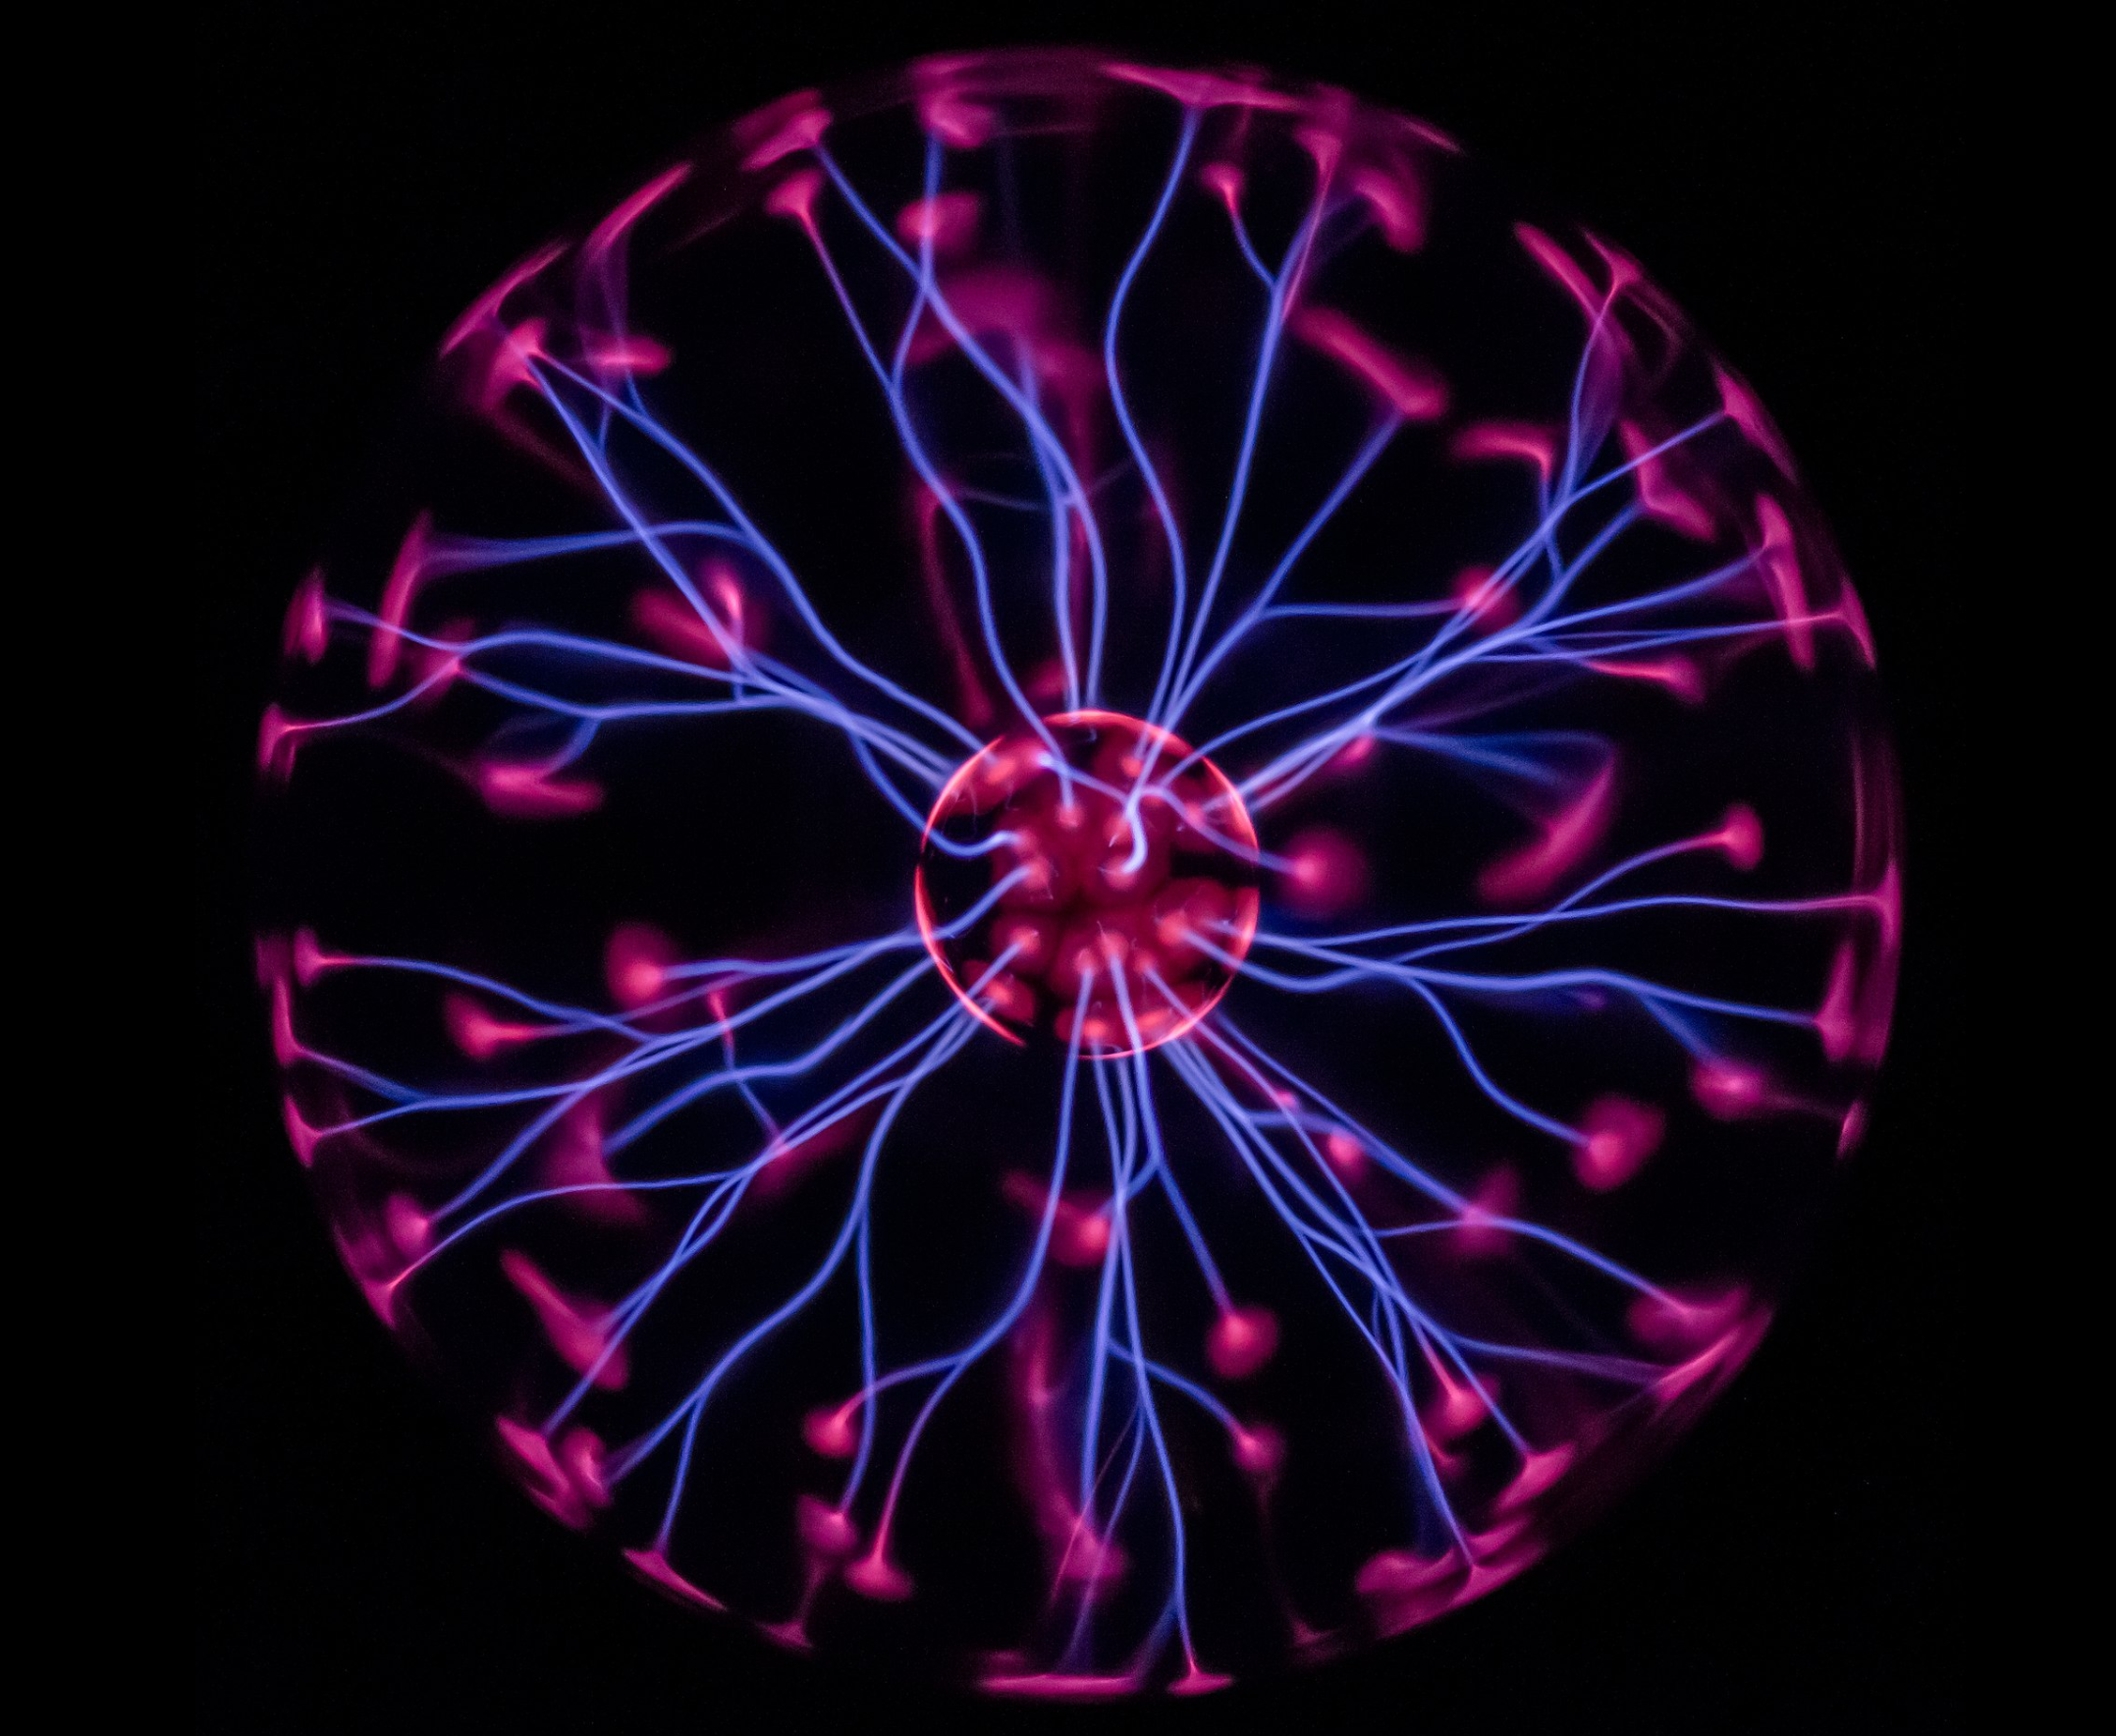
\includegraphics[width=.8\textwidth]{figures/plasma_ball.png}
    \caption{I think this would be a good thing to mention with the periodic cavity example. Pretty obvious relative homology classes.}
\end{figure}

Some notes from February '22
\begin{itemize}
    \item Colin: It is probably worth reading Gross--Kotiuga \cite{gross_electromagnetic_2004}, specifically starting at page 99 and seeing what more we can do then they do. They mention Greenberg--Harper \url{http://aix1.uottawa.ca/~rblute/COURSE2/Greenberg-Harper.pdf} for Alexander duality. Gross--Kotiuga really don't think about 4 dimensional topology at all though. I think that is where we have room to do quite a bit more. All the duality theorems are still readily usable. We should be able to extract anything they do from the 4d theory. Likewise, their work doesn't really seem to \emph{do} anything as far as circuits/measurement go with the topology. So that's actually still useful. They do get into FEM methods which could maybe be useful some day for plasma related problems.
    \item Colin: I think we should reach out to Kotiuga.
    \item Colin: I've also written some stuff about Ohmic materials that may be interesting here.
    \item Colin: In 4d, are there any interesting monogenic spinor fields?
    \item The LES is physical.
    \item Kunneth theorem may also be physical.
    \item What the heck... what about excision, mayer vietoris? 
    \item Alexander duality and image charges. I think alexander duality would let you study the fields outside of conductors. For example in 3d, electric fields are relative first homology classes on the complement of a conductor. A magnetic field induces a "dual" current in the conductor. Are these somehow absolute first homology classes? Also, we tend to take the physical postulate that charges sit on the boundary of currents.
    \item What about stratified spaces? There, the homology/cohomology may not be as "symmetric"
    \item Survey of cohomological physics -- Stasheff. Reach out to him? \clay{I know Stasheff a little bit, but maybe Alan does, too?}
    \item Colin: Does taking the homotopy class of the support of a field give a map from closed fields to cycles?
\end{itemize}

Some notes from 12/14/21
\begin{itemize}
    \item Who is the intended audience? How much detail? 
    \item Measurement devices and how they work in certain ways. Volt meter (0 current?), current meter (1 current?), ohm meter is some kind of combination of both (a pairing?)
    \item "on the mathematical foundations of electrical circuit theory"  \url{https://projecteuclid.org/journals/journal-of-differential-geometry/volume-7/issue-1-2/On-the-mathematical-foundations-of-electrical-circuit-theory/10.4310/jdg/1214430827.full}
    \item permeability and permitivity play the same role as resistance in the duality?
    \item Different coefficient rings?
    \item only access to $\partial M$. What can this tell you in the LES?
    \item \url{https://ncatlab.org/johnbaez/show/Circuit+theory}
    \item interesting 4-manifolds? Interesting 3 manifold $\times S^1$. List of ones that physicists use. Ideally with some boundary. Black hole/worm hole schwarzchild metric.
    \item \url{https://www.sciencedirect.com/science/article/abs/pii/0003491657900490}
    \item Foliations. Reeb foliation (can't be level surfaces to a charge distribution but it could for a magnetic potential?? I am lost on this one) and potential fields?
    \item Hodge star is the only place where geometry shows up.
\end{itemize}

% \begin{abstract}
% Motivated by the topological electromagnetism, we examine the de Rham homology and cohomology of smooth manifolds. We begin by constructing smooth multivector fields as sections of Clifford bundles and formulating the dual elements as distributional multivectors. The boundary operator is found to be the grade lowering portion of the gradient and the coboundary operator (or exterior derivative) is the grade raising portion. We give a concrete realization of  the cup product, cap product, and Poincar\'e dual map in terms of multivectors.
% \colin{Here's a comment from Colin.}
% \clay{Here's a comment from Clay.}
% \michael{Here's a comment from Michael.}
% \end{abstract}


\newpage
% %---------------------------------------------------------------------------------------------------------------------------
% \section{Introduction}
% %---------------------------------------------------------------------------------------------------------------------------
% \alan{electromagnetism is never mentioned outside of the abstract and a comment below. it is fair to mention that paper I burdened you with and the overall lack of de Rham homology material out there, which is why this must exist.}When working with the homology and cohomology of manifolds there one can choose to work with the notions of simplicial, singular, and de Rham theories, but they all end up equivalent, just with their own interpretation. It is a classical result that the simplicial and singular theories are equivalent\colin{put a source like hatcher here}. The de Rham theorem proves that singular cohomology over $\R$ is isomorphic to the de Rham cohomology of differential forms. Poincar\'e duality relates the de singular cohomology to the singular homology of the manifold and along with \cite[Theorem 2]{giaquinta_cartesian_1998} we can find an isomorphism between singular homology and the homology of de Rham currents, i.e., de Rham homology \cite{lekhyananda_homology_nodate}. 

% On the space of smooth multivector fields there exists a natural chain and cochain map which arise from the grade lowering $\grad  \cdot$ and grade raising component $\grad \wedge$ resp. of the gradient (or Dirac operator) $\grad$. There is a natural isomorphism between \alan{source plz}multivectors and forms and it is clear that the de Rham cohomology is isomorphic to the cohomology of $\grad \wedge$ since this operator corresponds to the exterior derivative $d$. It is also true that the homology of $\grad \cdot$ corresponds to the homology of $\delta$ as well but, by Hodge duality, this homology just reverses the indices of the de Rham cohomology. In this setting, the notion of the \alan{source plz}cup and cap products are clear as well. One could also choose to study the operator $\grad$ itself to see Hodge theory \cite{schwarz_hodge_1995}.


% The space of currents is dual to the space of multivector fields and it follows that the space is larger. Each multivector field can be realized as a current, but there are currents that are not multivector fields. The canonical example of such a current would be the Dirac mass $\delta_x$ which measures a field $f$ at a point $\delta_x[f]=f(x)$. Thinking of currents as measurements of fields allows us to relate these objects to physical devices used in electromagnetism. What does the homology of currents tell us about our measurement devices?
% \alan{is there a tag-line for currents that we can throw in here? something intuitive as these seem to be less common. Not sure what this is -- a continuous functional on the forms -- I would not mention distributions.  see \url{https://mathoverflow.net/questions/127128/why-are-currents-named-currents}}. 
%---------------------------------------------------------------------------------------------------------------------------


\section{Preliminaries}
\label{sec:preliminaries}
%---------------------------------------------------------------------------------------------------------------------------
We address only the necessary preliminaries here, though more detail can be found in various sources, for instance from Doran and Lasenby \cite{doran_geometric_2003}, and Hestenes and Sobczyk \cite{hestenes_clifford_1984}. These will include the basics of Clifford algebras with two key examples, foundations of the Clifford analysis of the Hodge--Dirac operator, and the notion of algebraic currents.

\subsection{Clifford Algebras}
\label{subsec:clifford_algebras}

To construct any Clifford algebra, take an $n$-dimensional vector space $V$ over a field $\mathbb{F}$ with quadratic form $Q$. By the polarization identity, given a $Q$ there is a unique corresponding symmetric bilinear form $g$. For more information on vector spaces with quadratic or bilinear forms, please see \cite{roman_metric_2008}. The tensor algebra is $\bigoplus_{n \in \mathbb{N}} V^{\otimes^n}$ and the Clifford algebra $\clifford(V,Q)$ is given by the quotient
\begin{equation}
\label{eq:ideal_quotient}
\clifford(V,Q) \coloneqq \bigoplus_{n \in \mathbb{N}} V^{\otimes^n} ~ / ~ \langle \blade{v} \otimes \blade{v} - Q(\blade{v}) \rangle
\end{equation}
with the induced addition and multiplication from the tensor algebra. For sake of clarity, we will think of $\clifford(V,Q)=\clifford(V,g)$ as needed, though most define Clifford algebras only using quadratic forms. Elements of $\clifford(V,Q)$ are referred to as \emph{multivectors}. When we take the totally singular form $Q=0$, the corresponding Clifford algebra is the exterior algebra $\bigwedge(V) = \clifford(V,0)$, and otherwise $\bigwedge(V)\subseteq C\ell(V,Q)$ as a subalgebra. Note that $\clifford(V,Q)$ is a $\mathbb{F}$-vector space of dimension $2^{n}$. For the remainder of this paper, we take $\mathbb{F}=\R$.

Given linearly independent vectors $\blade{v}_1,\dots,\blade{v}_k$ and the exterior product $\wedge$, an element of the form
\begin{equation}
    \blade{A_k} = \blade{v}_1 \wedge \cdots \wedge \blade{v}_k
\end{equation}
is a \emph{$k$-blade}, which are the simplest multivectors. Using the $\wedge$ inherently removes lower grade elements and keeps only the highest grade element (grade-$k$) of the product $A=\blade{v}_1\blade{v}_2\cdots \blade{v}_k$ since, at the very least, the product of two vectors yields \cref{eq:product_of_vectors}. This multivector $A$, often called a \emph{versor} since it is a product of vectors, is a sum of different graded elements called \emph{$k$-vectors}. A $k$-vector is a linear combination of $k$-blades and we denote this subspace of grade-$k$ elements by $\clifford^k(V,Q)$. Therefore, we have the direct sum decomposition
\begin{equation}
    \label{eq:grade_decomposition}
    \clifford(V,Q)= \bigoplus_{k=0}^n \clifford^k(V,Q).
\end{equation}
Some may refer to $k$-blades as \emph{simple} or \emph{decomposable} $k$-vectors as they correspond to rank-1 tensors in the tensor algebra. Moreover, they are also representative of subspaces which we discuss later. We write $\clifford^{k\oplus \ell}(V,Q)$ to represent the direct sum space of $k$- and $\ell$-vectors. A basis $\blade{e}_i$ of $V$ induces a $k$-blade basis by taking $\mathcal{I}=\{i_1,\dots,i_k\}$ to be a list of increasing indices $i_1 < \cdots < i_k$ and putting
\begin{equation}
\label{eq:basis_blades}
\blade{E}_\mathcal{I} \coloneqq \blade{e}_{i_1}\wedge \cdots \wedge \blade{e}_{i_k}.
\end{equation}

Some graded elements have special names. We say grade-0 objects are \emph{scalars}, grade-1 are \emph{vectors}, grade-2 are \emph{bivectors}, and grade-$n$ objects are \emph{pseudoscalars}. Typically, objects of grade-$(n-k)$ receive the prefix ``pseudo'', for example, we have pseudoscalars of grade-$(n-0)$ and \emph{pseudovectors} of grade-$(n-1)$. Multivectors also split into even and odd grades. We will work with the even-graded elements called \emph{spinors} as they form their own subalgebra $\clifford^+(V,Q)$. Given the direct sum decomposition in \cref{eq:grade_decomposition}, a multivector $A\in \clifford(V,Q)$ is given by
\begin{equation}
    \label{eq:grade_decomp_of_multivector}
A = \sum_{k=0}^n A_k
\end{equation}
where $A_k \in \clifford(V,Q)^k$.

One purpose of using a Clifford algebra $\clifford(V,Q)$ is to extend the exterior algebra $\bigwedge(V)$ to include a useful interior multiplication. Given $\blade{v},\blade{w}\in \clifford(V,Q)^1$, their product splits as
\begin{equation}
\label{eq:product_of_vectors}
    \blade{v}\blade{w}= \underbrace{\blade{v}\cdot \blade{w}}_{\textrm{grade-0}} +\underbrace{\blade{v}\wedge \blade{w}}_{\textrm{grade-2}},
\end{equation}
where $\cdot$ is the \emph{interior product}, in general, the lowest grade term of the product. However, for general Clifford algebras, we may have \emph{degenerate} vectors $\blade{v}$ such that for any other vector $\blade{w}$, $\blade{v}\cdot \blade{w}=0$. We will want to rid of this case.

To remove degenerate vectors from the algebra, we can force the quadratic form $Q$ to be completely nonsingular. We refer to such a Clifford algebra as a \emph{geometric algebra} and we write $\G = \clifford(V,Q)$ to denote such an algebra. To see more reasoning of calling such algebras ``geometric'', we again refer the reader to the chapter \cite{roman_metric_2008}. Using the vector space basis, we can determine the coefficients of the bilinear form by
\begin{equation}
g_{ij}=g(\blade{e}_i,\blade{e}_j)=\blade{e}_i \cdot \blade{e}_j.
\end{equation}
Let us quickly remark that if we were considering a Clifford algebra that was not a geometric algebra, then the matrix $g_{ij}$ of the bilinear form would be singular. We will carry on the rest of this paper working solely with geometric algebras for this reason, so the reader can assume that we take $g$ who, as transformations, are full rank.

Given a $k$-vector $A_k$ and an $\ell$-vector $B_\ell$, the product is
\begin{equation}
\label{eq:general_clifford_multiplication}
A_k B_\ell = \proj{|k-\ell|}{A_k B_\ell} + \proj{|k-\ell|+2}{A_k B_\ell} + \cdots + \proj{k+\ell}{A_k B_\ell},
\end{equation}
where the brackets $\proj{k}{-} \colon \G \to \G^k$ denote projection into the grade-$k$ subspace by
\begin{equation}
\proj{k}{A}=A_k
\end{equation}
when $A$ is given by \cref{eq:grade_decomp_of_multivector}. We define the \emph{(left) contraction} $A_k \contract B_\ell \coloneqq \proj{\ell-k}{A_k B_\ell}$. In general, the lowest grade term of $A_kB_\ell$ is the interior product $A_k \cdot B_\ell = \proj{|k-\ell|}{A_kB_\ell}$ and the exterior product $\wedge$ is the highest grade term of the product so that $A_k \wedge B_\ell = \proj{k+\ell}{A_k B_\ell}$. For a vector $\blade{v}$ we have $\blade{v}\cdot A = \blade{v}\contract A$ so many equations can be written with either $\cdot$ or $\contract$. Most will be written with $\contract$ as it is algebraically and geometrically more convenient. For notational simplicity, we also remove the subscript when projecting into the scalar subspace, $\proj{}{-}=\proj{0}{-}$, but this should not be confused with the notation for the ideal generated by a relation used only in \cref{eq:ideal_quotient}.

The \emph{reciprocal basis vectors $\blade{e}^i$} are those that satisfy $\blade{e}^i \cdot \blade{e}_j = \delta^i_j$. Reciprocal basis elements allow us to use the Riesz representation in order to avoid extraneous use of dual space elements since we are able to capture this functionality through the interior product. For sake of clarity, $\blade{e}^i \cdot \blade{e}^j = g^{ij}$ is the matrix inverse to $g_{ij}$ and $\blade{e}^i = g^{ij} \blade{e}_j$ are just the ``raised up'' indices. For a basis blade $\blade{E}_\mathcal{I}$, the reciprocal blade is $\blade{E}^\mathcal{I}$ and it satisfies the equation $\blade{E}^\mathcal{I} \cdot \blade{E}_\mathcal{J}= \delta^\mathcal{I}_\mathcal{J}$ where $\delta^\mathcal{I}_\mathcal{J}=1$ only when the sets of indices $\mathcal{I}$ and $\mathcal{J}$ are identical.

Geometric algebras have a bilinear product $\G \times \G \to \R$ called the \emph{multivector inner product} which is given by
\begin{equation}
(A,B) \coloneqq \proj{}{A^\dagger B}.
\end{equation}
This equation is given in terms of the \emph{reverse operator} $\dagger$ which for $\lambda \in \R$ satisfies
\begin{equation}
(A+B)^\dagger=A^\dagger + B^\dagger, \quad (\lambda A)^\dagger = \lambda^\dagger A^\dagger = \lambda A^\dagger, \quad A^{\dagger \dagger}=A, \quad (AB)^\dagger = B^\dagger A^\dagger,
\end{equation}
and on a versor we have
\begin{equation}
    (\blade{v}_1\blade{v}_2 \cdots \blade{v}_k)^\dagger \coloneqq \blade{v}_k \cdots \blade{v}_2 \blade{v}_1.
\end{equation}
Note that $\dagger$ acts as the adjoint in the product $(-,-)$ which follows from the cyclic property of the scalar grade projection \cite[eq. (138)]{chisolm_geometric_2012}. To see this, we take another multivector $C$ and note
\begin{align}
(CA,B) = \proj{}{(CA)^\dagger B} = \proj{}{ A^\dagger C^\dagger B } = (A,C^\dagger B),
\end{align}
We define a semi-norm $|-|^2\coloneqq (-,-)$ called the \emph{multivector norm}. If $|A|=\pm 1$ we say that $A$ is \emph{unit}. It is worth saying that for a multivector field written in terms of basis blades $f=\sum_{\mathcal{I}} f_\mathcal{I} \blade{E}_\mathcal{I}$ that
\begin{equation}
\label{eq:inner_product_with_basis}
f_\mathcal{I} = (f, \blade{E}^\mathcal{I}),
\end{equation}
so long as the quadratic form is definite (e.g., the quadratic form is the Euclidean norm). We also have that
\begin{equation}
\blade{E}^\mathcal{I} = (\blade{e}^{i_1} \wedge \cdots \wedge \blade{e}^{i_k})^\dagger.
\end{equation}

There exists a vector basis for $V$ where $p$ vectors square to $-1$ and $q$ vectors square to $+1$ and $p+q=n$. The corresponding geometric algebra is often written as $\G_{p,q}$. We will focus most on the the case where $Q$ is positive definite and to distinguish this, we can write $\G_n$ if it is necessary. For $\G_n$, the multivector inner product and multivector norm are both positive definite. One can see that the multivector inner product treats the space $\G_n$ as a $2^n$-dimensional inner product space with a basis given by the blades $\blade{E}_\mathcal{I}$. \Cref{eq:inner_product_with_basis} just specifies that we have chosen a set of blades orthonormal with respect to the multivector inner product.

If the basis $\blade{e}_i$ is orthonormal in $V$, then the set of basis blades $\blade{E}_\mathcal{I}$ are orthonormal versors in $\G_n$ since
\begin{equation}
\blade{E}_\mathcal{I} = \blade{e}_{i_1}\wedge \cdots \wedge \blade{e}_{i_k} = \blade{e}_{i_1} \blade{e}_{i_2} \cdots \blade{e}_{i_k}.
\end{equation}
Their products become much clearer to compute. We have
\begin{equation}
\blade{E}_\mathcal{I} \blade{E}_\mathcal{J} =  \pm \blade{E}_{\mathcal{I}\triangle \mathcal{J}},
\end{equation}
where $\triangle$ is the symmetric difference of the sets $\mathcal{I}$ and $\mathcal{J}$ and the $\pm$ is used solely due to the fact that vectors $\blade{e}_i$ comprising the versors $\blade{E}_\mathcal{I}$ may need to be swapped and
\begin{equation}
-\blade{E}_\mathcal{I} = \blade{e}_{i_1} \blade{e}_{i_2} \cdots \blade{e}_{i_{j+1}} \blade{e}_{i_j}\cdots \blade{e}_{i_k}.
\end{equation}
For a concrete example, take $\blade{E}_{123}=\blade{e}_1\blade{e}_2\blade{e}_3$ and $\blade{E}_{124}$ both in $\G_n$, then
\begin{equation}
\blade{E}_{123}\blade{E}_{124}= \blade{e}_1\blade{e}_2\blade{e}_3\blade{e}_1\blade{e}_2\blade{e}_4=\blade{e}_1\blade{e}_2\blade{e}_1\blade{e}_2\blade{e}_3\blade{e}_4 = -\blade{e}_1\blade{e}_2\blade{e}_2\blade{e}_1\blade{e}_3\blade{e}_4 = -\blade{e}_1\blade{e}_1\blade{e}_3\blade{e}_4 = -\blade{E}_{34}.
\end{equation}
Using an orthonormal vector basis shows how nicely versors act algebraically. Multiplication is just reduction of words in the characters $\blade{e}_i$ subject to the relations $\blade{e}_i^2=1$ and where swaps add a sign $\blade{e}_i\blade{e}_j=-\blade{e}_j\blade{e}_i$.

\begin{remark}
Though we will not cover the content here, it is worth mentioning that versors in a geometric algebra $\G_{p,q}$ form a group under multiplication called the \emph{Clifford group} and the unit versors define the \emph{spin group} $\mathrm{Spin}(p,q)$. The algebra of bivectors in $\G_{p,q}$ with the commutator $[-,-]$ (often written as $\times$ as well) is the Lie algebra $\mathfrak{spin}(p,q)$.
\end{remark}

Geometric algebras also have a unique isomorphism $\perp \colon \G^k \to \G^{n-k}$ and this $\perp$ is equivalent to the Hodge star $\star$ in $\bigwedge(V)$. To construct this isomorphisms, we first take an arbitrary basis for $V$ and build the volume element
\begin{equation}
    \mu \blade{I} \coloneqq \blade{e}_1 \wedge \cdots \wedge \blade{e}_n,
\end{equation}
where the unit blade $\blade{I}$ is the \emph{unit pseudoscalar} and $\mu$ represents the volume scaling. Note that $\blade{I}$ represents the subspace $V$ and for geometric algebras it defines the \emph{dual}
\begin{equation}
\label{eq:dual}
A^\perp \coloneqq A\pseudoscalar^{-1}.
\end{equation}
For example, if $\blade{v}$ is a vector then we have $\blade{v}^\perp$ is a pseudovector representing a scaled copy of the hyperplane perpendicular to $\blade{v}$.

Moreover, the dual allows for exchanging products
\begin{equation}
(A\contract B)^\perp = A\wedge B^\perp
\end{equation}
and the exterior product
\begin{equation}
(A\wedge B)^\perp = A\contract B^\perp
\end{equation}
and helps elucidate the geometrical meaning of $\contract$ and $\wedge$ (see \cite{chisolm_geometric_2012}). Finally, it is worth saying that in $\G_n$ we have $\pseudoscalar^{-1}=\pseudoscalar^\dagger$.

Given a subspace $U\subset V$ in a space with nonsingular $Q$, we can put $V=U \oplus U^\perp$. In much the same way, given a unit $k$-blade $\blade{U_k}$ we can find a decomposition of $\pseudoscalar$ by $\pseudoscalar = \blade{U_k}\wedge \blade{U_k}^\perp$. Actually, multiplication in $\G$ allows for projection onto subspaces using this identification.
\begin{definition}
Given an multivector $B$ and unit $k$-blade $\blade{U_k}$, the \emph{projection} onto the subspace $\blade{U_k}$ is
\begin{equation}
\label{eq:projection}
\projection_{\blade{U_k}}(B) \coloneqq (B\contract \blade{U_k}) \blade{U_k}^{-1}.
\end{equation}
\end{definition}
The projection preserves grades $\projection_{\blade{U_k}}(B_\ell)\in \G^\ell$. 

\begin{example}
Rather than a sequence of multiple examples, it will prove to be far more illuminating to construct one large example for which most of the preliminaries to this point can be used in a meaningful way. As such, we shall not rule out the utility that other areas may gain out of using geometric algebras with pseudo inner products even though this paper is predominantly concerned with the positive definite case. The classical example is the \emph{spacetime algebra} defined by taking $V=\R^4$ with a vector basis $\blade{e}_0,\blade{e}_1,\blade{e}_2,\blade{e}_3$ satisfying
\begin{subequations}
\begin{align}
\blade{e}_0 \cdot \blade{e}_0 &= -1\\
\blade{e}_0 \cdot \blade{e}_i &= 0  &i=1,2,3\\
\blade{e}_i \cdot \blade{e}_j &= \delta_{ij}, &i,j=1,2,3.
\end{align}
\end{subequations}
We refer to $\blade{e}_0$ as \emph{temporal} since its square is negative and $\blade{e}_i$ for $i=1,2,3$ are \emph{spatial} since their squares are positive. For this basis, the matrix for this inner product in this basis assumes the form $\eta =\operatorname{diag}(-1,~ +1,~ +1,~+1)$ (often called the \emph{Minkowski metric}). The associated quadratic form $Q$ can be found from $\eta$ by polarization. For a spacetime vector $\blade{v} = v_0 \blade{e}_0 +v_1 \blade{e}_1 + v_2 \blade{e}_2 + v_3 \blade{e}_3$,
\begin{equation}
\label{eq:spacetime_inner_product}
|\blade{v}|^2 = (\blade{v},\blade{v}) = \blade{v} \cdot \blade{v} = -v_0^2 + \sum_{i=1}^3 v_i^2.
\end{equation}
It is clear that the norm is definite when all vectors are spatial, but in the case of spacetime there are null vectors $\blade{c}$ such that $|\blade{c}|=0$. For example, $\blade{c}=\blade{e}_0 + \blade{e}_1$. The collection of null vectors define the light cone in Minkowski space. Also, it is important to distinguish these null vectors from degenerate vectors. Though $\blade{c}$ is null, it is not true that for any $\blade{c}$ and all other vector $\blade{v}$ that $\blade{c} \cdot \blade{v}=0$.

As the notation above suggests, the geometric algebra of Euclidean space $\R^3$, $\G_3$, should naturally appear inside of the spacetime algebra. The spatial \emph{trivector} $\blade{e}_1 \blade{e}_2 \blade{e}_3$ is unit
\begin{equation}
|\blade{e}_1 \blade{e}_2 \blade{e}_3| = \sqrt{\proj{}{(\blade{e}_1 \blade{e}_2 \blade{e}_3)^\dagger \blade{e}_1 \blade{e}_2 \blade{e}_3}} = \sqrt{\proj{}{\blade{e}_3 \blade{e}_2 \blade{e}_1 \blade{e}_1 \blade{e}_2 \blade{e}_3}}=1
\end{equation}
and represents the spatial subspace $\mathrm{Span}(\blade{e}_1, \blade{e}_2, \blade{e}_3) \subset \R^4$. With slight abuse of notation, the projection of $\G_{1,3}$ onto this subspace yields
\begin{equation}
\projection_{\blade{e}_1 \blade{e}_2  \blade{e}_3}(\G_{1,3}) = \G_3.
\end{equation}
In $\G_3$, we can specify an arbitrary multivector $A$ by
\begin{equation}
A= a_0 + a_1 \blade{e}_1 + a_2 \blade{e}_2 + a_3 \blade{e}_3 + a_{12} \blade{e}_1\blade{e}_2 + a_{13} \blade{e}_1\blade{e}_3 + a_{23} \blade{e}_2\blade{e}_3 + a_{123} \blade{e}_1 \blade{e}_2 \blade{e}_3.
\end{equation}
It will be pertinent later to define $\bivector_{ij}\coloneqq \blade{e}_i\blade{e}_j$ for $i\neq j$. Using this substitution, the grade projections read
\begin{subequations}
\begin{align}
\proj{}{A}&=a_0\\
\proj{1}{A}&=a_1 \blade{e}_1 + a_2 \blade{e}_2 + a_3 \blade{e}_3\\
\proj{2}{A}&=a_{12} \blade{B}_{12} + a_{13} \blade{B}_{13} + a_{23} \blade{B}_{23}\\
\proj{3}{A}&= a_{123} \blade{e}_1  \blade{e}_2 \blade{e}_3.
\end{align}
\end{subequations}
Hence, we can write a spinor as
\begin{equation}
A_+ = a_0 + a_{12} \blade{B}_{12} + a_{13} \blade{B}_{13} + a_{23}\blade{B}_{23}.
\end{equation}
Note as well that the spatial unit 2-blades always satisfy
\begin{align}
\blade{B}_{23}^2 = \blade{B}_{13}^2 = \blade{B}_{12}^2 = -1
\end{align}
and we find that
\begin{equation}
\blade{B}_{23}\blade{B}_{13}\blade{B}_{12} = -1.
\end{equation}
Hence, the even subalgebra $\G_3^+$ isomorphic to the quaternion algebra $\quat$ by
\begin{equation}
\mathbf{i} \leftrightarrow \blade{B}_{23}, \quad \mathbf{j} \leftrightarrow \blade{B}_{13}, \quad \mathbf{k} \leftrightarrow \blade{B}_{12}
\end{equation}
Given a quaternion, there is an equivalent spinor $A_+$; the imaginary part of the quaternion corresponds to the grade two part of the spinor $\proj{2}{A_+}$.

We can project down one dimension further by $\projection_{\bivector_{12}} (\G_3) = \G_2$ and
we can verify quickly that
\begin{subequations}
\begin{align}
    \projection_{\blade{e}_1 \blade{e}_2}(A) =  a_0 + a_1 \blade{e}_1 + a_2 \blade{e}_2 + a_3 \blade{e}_3 + a_{12} \bivector_{12}.
\end{align}
\end{subequations}
Given that $\blade{B}_{12}^2=-1$ we can put $z \coloneqq x + y \blade{B}_{12} \in \G_2^+$ for $x,y\in \R$ which is exactly a representation of the complex number $\zeta = x+ \mathbf{i}y$ in $\C$ and $\mathbf{i}$ here can be thought of as the unit pseudoscalar in the plane. Again, the imaginary part is $\proj{2}{z}$.
\end{example}

% Using the interior product, we build the vector space dual elements by defining through the \emph{reciprocal basis} $\blade{e}^i$ by requiring $\blade{e}^i\cdot \blade{e}_j = \delta_{ij}$.
%
%The higher graded elements are generated from taking exterior products of linearly independent vectors, e.g.,

%Most generally, the multiplication of a $k$-vector $A_k$ and an $\ell$-vector $B_\ell$ is
%\begin{equation}
%\label{eq:general_clifford_multiplication}
%A_k B_\ell = \proj{|k-\ell|}{A_k B_\ell} + \proj{|k-\ell|+2}{A_k B_\ell} + \cdots + \proj{k+\ell}{A_k B_\ell},
%\end{equation}
%for which we define the \emph{(left) contraction}  $A_k \rfloor B_\ell \coloneqq \proj{|\ell-k|}{A_k B\ell}$ and note that for a vector $\blade{v}$ we have $\blade{v}\cdot A = \blade{v}\rfloor A$. We can see the subspace of even graded elements $\clifford^+(V,Q)$ forms a subalgebra often called the \emph{even subalgebra} whose elements are called \emph{spinors}. \colin{It may be worthwhile to say that spinors are really more general than this.} On multivectors, have the \emph{reverse} $\dagger$ which we define on a $k$-blade by
%\begin{equation}
%    \blade{A_k}^\dagger = \blade{v}_k\wedge \cdots \wedge \blade{v}_1 = (-1)^{k(k-1)/2} \blade{A_k}
%\end{equation}
%and extend linearly to multivectors.





%Clifford algebras whose quadratic form is inherited from an (pseudo)inner product $Q(-)=g(-,-)$ on $V$ are referred to as \emph{geometric algebras}. Since $g$ will be arbitrary or clear from context we put $\G\coloneqq \clifford(V,g)$ and also assume that our geometric algebras are taken to be solely over the field $\R$. When $V$ has pseudo-euclidean inner product with $p$ vectors that square to $-1$ (temporal) and $q$ that square to $+1$ (spatial), we will put $\G_{p,q}$ and assume $p+q=n$. With an arbitrary basis $\blade{e}_i$,
%\begin{equation}
%\blade{e}_1 \wedge \cdots \wedge \blade{e}_n = \sqrt{(-1)^p \det g} \blade{I}.
%\end{equation}


\subsection{Clifford Analysis}
\label{subsec:clifford_analysis}

Given a smooth semi-Riemannian manifold $M$ with metric tensor field $g$ and boundary $\partial M$, each tangent space $T_xM$ can be made into a geometric algebra $\G_x M \coloneqq C\ell(T_xM,g_x)$ and we call $\G_xM$ the \emph{geometric tangent space}. The geometric tangent spaces are glued together to form the geometric algebra bundle $\G M\coloneqq \bigsqcup_{x\in M}\G_x M$. We will call the $C^\infty$ sections of this bundle $\smoothfields{M}{\G}$ the \emph{smooth multivector fields} and the continuous sections $\contfields{M}{\G}$ the \emph{continuous multivector fields}. Let $\nabla$ be the Levi--Civita connection on $M$. Then for a vector field $\blade{v}$ we have the covariant derivative $\nabla_{\blade{v}}$ which is extended to multivector fields, e.g., by \cite{schindler_geometric_2020}. Given local coordinates $x^i$ on $M$ we have the induced (gradient) basis $\blade{e}_i(x)\in \G_xM$. Suppressing the pointwise notation, $\blade{e}_i\cdot \blade{e}_j = g_{ij}$. Also in the tangent space are the reciprocal vectors $\blade{e}^i$ which are Riesz representatives corresponding to the dual basis $dx^i$ since $dx^i(\blade{e}_j) = \blade{e}^i \cdot \blade{e}_j$. We will not get rid of the dual basis entirely since we still find use for the elements as coordinate measures in integration. Basis blades $\blade{E}_\mathcal{I}$ and their reciprocals $\blade{E}^\mathcal{I}$ carry over to each tangent space as well.

The \emph{Hodge--Dirac operator} (or \emph{gradient}) $\grad$ in these coordinates is
\begin{equation}
    \grad \coloneqq \sum_{i=1}^n \blade{e}^i \nabla_{\blade{e}_i}.
\end{equation}
This derivative acts algebraically as a vector and
\begin{equation}
\label{eq:grad_of_planespinor}
\grad f = \grad \contract f + \grad \wedge f.
\end{equation}
In particular, $\grad \wedge$ is equivalent to the exterior derivative $d$ on differential forms $\Omega(M)$, $\grad \contract$ is equivalent to the codifferential $\delta$, and $\grad^2 = \Delta$ is the Laplace--Beltrami operator. The kernel of $d+\delta$ on $\Omega^k(M)$ is coupled to the (co)homology of $M$ and so $\grad$ retains this property as well. This relationship of the analysis of $d+\delta$ (and equivalently $\grad$) to the absolute and relative (co)homology of $M$ is formalized in Hodge theory and is useful for proving existence and uniqueness for boundary value problems \cite{schwarz_hodge_1995}. However, in Clifford analysis, it is commonplace to consider mixed grade multivectors also in the kernel of $\grad$. This space is far bigger since we find that grades can ``mix'' together. For example, take $f_+ = f_0 + f_2 \bivector$ in defined on the unit disk $\mathbb{D} \subset \R^2$ and $\bivector$ is the unit bivector field then
\begin{equation}
\grad f_+ = \grad \wedge f_0 + \grad \contract ( f_2 \bivector).
\end{equation}
If we considered only singly graded elements such as the scalar fields $f_0$ or bivector fields $f_2 \bivector$ on their own, then the only elements in $\ker \grad$ are constant fields. Combine them together into a spinor field $f_+ \in \G^+(\R^2)$ and this can now be any holomorphic function such as $z=x^1+x^2\bivector$ or even any power series in $z$ which we will revisit later. Since this space is far bigger, it can be used to extract more topological data about $M$, namely the homeomorphism type, as we see in \cref{thm:gelfand}.

\begin{definition}
Let $f\in \smoothfields{M}{\G}$, then we say that $f$ is \emph{monogenic} if $\grad f = 0$. We denote the space of monogenic fields by $\monogenics(M)$.
\end{definition}

Monogenic fields are the emphasis of Clifford analysis and many of the theorems of holomorphic functions in complex analysis apply to these fields. Once again, on the unit disk $\mathbb{D}$ take $f_+ = f_0 + f_2 \bivector$ then if $\grad f_+ =0$ we can use \cref{eq:grad_of_planespinor} to derive the Cauchy--Riemann equations
\begin{align}
\label{eq:cauchy_riemann_equations}
\frac{\partial f_0}{\partial x^1} &= \frac{\partial f_2}{\partial x^2} & \frac{\partial f_0}{\partial x^2} &= -\frac{\partial f_2}{\partial x^1}
\end{align}
which shows the function $z$ is indeed monogenic. For more detail on the relationship of monogenic spinor fields to complex holomorphic functions see Doran and Lasenby \cite[\S 6.3.1]{doran_geometric_2003}.

Since $\grad$ is grade-1, we have $\grad \colon \smoothfields{M}{\G^{\pm}} \to \smoothfields{M}{\G^\mp}$ which yields the direct sum decomposition
\begin{equation}
    \monogenics(M) = \monogenics^+(M) \oplus \monogenics^-(M).
\end{equation}
We can note that each of the graded components of $f_+\in \monogenics^+(M)$ are also harmonic $\Delta \proj{2k}{f_+}=0$. Also, the fact that a product of spinor fields is again a spinor field will make it more convenient to work with $\monogenics^+(M)$ instead of the whole of $\monogenics(M)$. 

In order to integrate, we build differential forms from $k$-vector fields by attaching a measure. Take the coordinate measures (dual basis in the cotangent space) $dx^i$ in local coordinates and multiply by the corresponding reciprocal vector to get \emph{basic directed measures} $d\blade{x}^i = \blade{e}^i dx^i$ (no summation implied), which determine the \emph{$k$-dimensional directed measures}
\begin{equation}
    dX_k \coloneqq \frac{1}{k!} \sum_{i_1 < \cdots < i_k} d\blade{x}^{i_1}\wedge \cdots \wedge d\blade{x}^{i_k} = \frac{1}{k!} \sum_{\mathcal{I}} \blade{E}^{\mathcal{I}^\dagger} dx^{\mathcal{I}}
\end{equation}
An arbitrary differential $k$-form $\alpha_k$ is given by taking a corresponding $k$-vector $A_k$ and contracting along the $k$-dimensional directed measure
\begin{equation}
\alpha_k = A_k \contract dX_k^\dagger.
\end{equation}
Specifically, $A_k = \sum_{\mathcal{I}} \alpha^{\mathcal{I}} \blade{E}_{\mathcal{I}}$ is called the \emph{multivector equivalent of $\alpha_k$}. This is a realization of the isomorphism between $\smoothfields{M}{\G}$ and $\Omega(M)$ as $C^\infty(M)$-modules and it can be viewed as an extension of the musical isomorphisms \cite[chapter 13]{lee_introduction_2012}. The multivector equivalent of the Riemannian volume form $\mu$ is $\pseudoscalar^{-1^\dagger}$ and $\blade{I}(x)$ represents the tangent space $T_x M$. Of course, in the case where $g$ is definite, the equivalent to $\mu$ is simply $\pseudoscalar$. On $\partial M$, we have the \emph{boundary pseuodoscalar} $\blade{I}_\partial$ and dual to this the boundary normal vector field $\normal = \pseudoscalar_\partial^\perp$. As on $M$, the boundary pseudoscalar $\blade{I}_\partial$ is the multivector equivalent of the boundary area form $\mu_\partial$. From this point forward, we work solely with multivector fields and contract with directed measures to integrate. We now realize the action of $\grad \wedge$ and $\grad \contract$ as the equivalents of $d$ and $\delta$ by
\begin{align}
d \alpha_k &= (\grad \wedge A_k) \contract dX_{k+1}^\dagger, & \delta \alpha_k &= (\grad \contract A_k)\contract dX_{k-1}^\dagger.
\end{align}

For smooth $r$-forms $\alpha_r$ and $\beta_r$, we have an $L^2$-inner product 
\begin{equation}
\int_M \alpha_r \wedge \star \beta_r 
\end{equation}
where $\star$ is the Hodge star. By definition, the Hodge star acts on $r$-forms by returning a Hodge dual $n-r$-form so that on the multivector equivalents we have
\begin{equation}
\alpha_r \wedge \star \beta_r  = \proj{}{A_r B_r^\dagger}\mu = (A_r,B_R)\mu
\end{equation}
as well as
\begin{equation}
    \alpha_r \wedge \star \alpha_r = |A_r|^2\mu.
\end{equation}
For the action of $\star$ on the multivector equivalents we will put $B_r^\star$ for which we have
\begin{equation}
B_r^\star = (\pseudoscalar^{-1} B_r)^\dagger
\end{equation}
and we can quickly verify that
\begin{align}
(A_r \wedge B_r^\star)\cdot dX_n^\dagger = (A_r\cdot B_r^\dagger) \pseudoscalar^{-1 \dagger}\cdot dX_n^\dagger = \proj{}{A_rB_r^\dagger}\mu.
\end{align}
This allows us to define can now define an $L^2$ inner product on multivector fields.
\begin{definition}
\label{def:multivector_field_inner_product}
Let $A$ and $B$ be multivector fields. Then the \emph{multivector field inner product} is defined by
\begin{equation}
\multivecinnerproduct{A}{B} \coloneqq \int_M (A,B) \mu.
\end{equation}
\end{definition}
If $\multivecinnerproduct{A}{B} = 0$, then we say $A$ and $B$ are orthogonal. Once again, this is only a definite inner product when $g$ is positive definite.  We put $\multivecinnerproduct{\cdot}{\cdot}_\partial$ to represent the inner product on the boundary manifold. Note that if we take a homogeneous $r$-vector field $A_r$ and $s$-vector field $B_s$ that if $s\neq r$, the multivector field inner product is zero. Hence, the orthogonal direct sum with respect to the $L^2$ multivector inner product agrees with the grade based direct sum. It will suffice to use the symbol $\oplus$ for both. One should view this as a slight extension to the $r$-form inner product that garners the ability to consider the inner product of elements that are not necessarily homogeneous in grade. The following proposition confirms this.
\begin{proposition}
Given two $r$-forms, the $r$-form inner product is equal to the multivector inner product on their corresponding multivector equivalents.
\end{proposition}
\begin{proof}
Let $\alpha_r$ and $\beta_r$ be $r$-forms with multivector equivalents $A_r$ and $B_r$ respectively. Then
\begin{align*}
    \int_M \alpha_r \wedge \star \beta = \int_M A_r \contract B_r^\dagger \mu = \int_M (A_r,B_r) \mu =\multivecinnerproduct{A_r}{B_r},
\end{align*}
by the definition of the Hodge star.
\end{proof}

\subsection{Boundary and Green's Formula}

\colin{This whole subsection is a mess because it is copy pasted}
This is pertinent when we take $M$ to be a manifold with boundary $\partial M$. In this case we let $\blade{I}_\partial$ denote the tangent $n-1$-blade and build boundary measure via
\begin{equation}
\mu_\partial \coloneqq \blade{I}_\partial^{-1} \cdot dX_{n-1}.
\end{equation}
The normal space is 1-dimensional and we put $\blade{\nu}$ to refer to the boundary normal space.

We will need to know whether a field is tangent or normal to the boundary $\partial M$.  First, let $\normal,\blade{e}_1,\dots,\blade{e}_{n-1}$ be an orthornormal vector basis for $\G_xM$ for $x\in \partial M$ and let $\blade{E}_\mathcal{I}$ be the orthornormal basis versors. Then, for any multivector $A\in \G_xM$ we have
\begin{equation}
\label{eq:tangent_normal_decomposition}
A = \sum_{\normal \in \mathcal{I}} A^{\normal \in \mathcal{I}} \blade{E}_{\normal \in \mathcal{I}} + \sum_{{\normal \notin \mathcal{I}} } A^{{\normal \notin \mathcal{I}}} \blade{E}_{\normal \notin \mathcal{I}} 
\end{equation}
where the notation $\normal \in \mathcal{I}$ means to consider only versors who have $\normal$ appear and $\normal \notin \mathcal{I}$ takes only those where $\normal$ does not appear. It is clear that $\pseudoscalar_{\partial} = \blade{e}_{1}\blade{e}_{2}\cdots \blade{e}_{n-1}$ and therefore
\begin{equation}
\label{eq:tangentpart}
\tangentpart A = \sum_{\normal \in \mathcal{I}} A^{\normal \in \mathcal{I}} \blade{E}_{\normal \in \mathcal{I}}
\end{equation}
and hence the normal part is clear
\begin{equation}
\label{eq:normalpart}
\normalpart A = \sum_{{\normal \notin \mathcal{I}} } A^{{\normal \notin \mathcal{I}}} \blade{E}_{\normal \notin \mathcal{I}} .
\end{equation}
Of course, this is all done pointwise, but it extends nicely to a field $A\in \G(M)$.

\begin{proposition}
Let $\alpha_s$ be an $s$-form defined on $M$ and let $\iota \colon R \to M$ be the inclusion of the submanifold $R$ into $M$. Then the pullback $\iota^*$ on the multivector equivalent $A_s$ is given by
\begin{equation}
\iota^* \alpha_s = \projection_{\blade{I}_R}(A_s) \cdot dX_s.
\end{equation}
\end{proposition}
\todo{This proof is super lengthy and really it should just use the fact that the pullback can be identified with the tangential part like in Schwarz}
\begin{proof}
Note that by definition we have
\[
(\iota^* \alpha_s)_x (\blade{v}_1,\dots,\blade{v}_r) = (\alpha_s)_x(d\iota_x\blade{v}_1,\dots, d\iota_x\blade{v}_r ),
\]
for arbitrary vector fields $\blade{v}_1,\dots,\blade{v}_s$ and at all $x\in R$. Then, since $\iota$ is inclusion, we have
\[
d\iota_x = \projection_{\blade{I}_R(x)},
\]
at each point $x \in R$ and hence
\[
\iota^* \alpha_s = \alpha_s \circ \projection_{\blade{I}_R}.
\]
For all $\blade{v}_i$ we can put
\[
\blade{v}_i = \projection_{\blade{I}_R}(\blade{v}_i) + \rejection_{\blade{I}_R}(\blade{v}_i),
\]
and note for the multivector equivalent
\begin{align}
\label{eq:previous_1}
(\projection_{\blade{I}_R}(A_s) \cdot dX_s)(\blade{v}_1,\dots,\blade{v}_s) &= (\projection_{\blade{I}_R}(A_s) \cdot dX_s)(\projection_{\blade{I}_R}(\blade{v}_1) + \rejection_{\blade{I}_R}(\blade{v}_1),\dots,\projection_{\blade{I}_R}(\blade{v}_s) + \rejection_{\blade{I}_R}(\blade{v}_s))\\
&= (\projection_{\blade{I}_R}(A_s) \cdot dX_s)(\projection_{\blade{I}_R}(\blade{v}_1),\dots,\projection_{\blade{I}_R}(\blade{v}_s)),
\end{align}
since $\projection_{\blade{I}_R}(A_s)$ is supported only on $R$. Then, if $s\leq r$,
\begin{align*}
\iota^*\alpha_s &= (A_s \cdot dX_s)(\projection_{\blade{I}_R}(\blade{v}_1),\dots,\projection_{\blade{I}_R}(\blade{v}_s))\\
&= ((\projection_{\blade{I}_R}(A_s) + \rejection_{\blade{I}_R}(A_s)) \cdot dX_s)(\projection_{\blade{I}_R}(\blade{v}_1),\dots,\projection_{\blade{I}_R}(\blade{v}_s))\\
&= (\projection_{\blade{I}_R}(A_s) \cdot dX_s)(\projection_{\blade{I}_R}(\blade{v}_1),\dots,\projection_{\blade{I}_R}(\blade{v}_s)),
\end{align*}
and by \cref{eq:previous_1} we have our intended result. If $s>r$, then 
\[
\iota^* \alpha_s = 0 = \projection_{\blade{I}_R}(A_s)
\]
which proves the proposition.
\end{proof}

The above seems to motivate the choice of \cite{schwarz_hodge_1995} to put $\tangentpart_R = \iota^*$ to refer to the tangential part of a differential form. The normal part of a form is $\normalpart_R \alpha_s = \alpha_s - \tangentpart_R \alpha_s$. The following corollary is immediate given \cref{eq:projection_rejection_duality,eq:projection+rejection_blade}. 
\begin{corollary}
Let $\alpha_s$ be an $s$-form with $s<r$ and $s<n-r$ and multivector equivalent $A_s$. Then
\begin{equation}
\normalpart_R \alpha_s = \alpha_s - \operatorname{P}_{\pseudoscalar_R}(A_s)\cdot dX_s^\dagger = \rejection_{I_R}(A_s)\cdot dX_s^\dagger.
\end{equation}
\end{corollary}

\colin{I should mention that $\contfields{\partial M}{\G}$ really consists of boundary traces of smooth fields on $M$}
\begin{proposition}
\label{prop:tangent_normal_proposition}
Let $\phi \in \G(\boundary)$, then 
\begin{enumerate}[i.]
\item $\phi \in \ker \tangentpart$ if and only if $\normal \contract \phi = 0$;
\item $\phi \in \ker \normalpart$ if and only if $\normal \wedge \phi = 0$.
\end{enumerate}
\end{proposition}
\begin{proof}
The proof is immediate given \cref{eq:tangentpart,eq:normalpart}. First, if $\phi \in \ker \tangentpart$ then $\phi = \normalpart \phi$ by \cref{eq:tangent_normal_decomposition}. Hence,
\begin{equation}
\normal \contract \phi = \sum_{{\normal \notin \mathcal{I}} } \phi^{{\normal \notin \mathcal{I}}} \normal \contract \blade{E}_{\normal \notin \mathcal{I}}
\end{equation}
but $\normal \contract \blade{E}_{\normal \notin \mathcal{I}} = 0$ and thus we have the first direction. On the other hand, if $\normal \contract \phi = 0$ then every $\phi^{\normal \in \mathcal{I}}=0$ which finishes the proof. The proof for (ii) is done \emph{mutatis mutandis}.
\end{proof}

\begin{proposition}
On multivector equivalents $A_{r-1}$ and $B_r$, we have Green's formula
\begin{equation}
\multivecinnerproduct{\grad \wedge A_{r-1}}{B_r} = \multivecinnerproduct{A_{r-1}}{\grad \contract B_r} + (-1)^{p} \int_{\partial M} (A_{r-1}\contract B_r^\dagger,  \blade{\nu}) \mu_\partial.
\end{equation}
\end{proposition}
\begin{proof}
First, we have
\begin{equation}
\int_M d(\alpha_{r-1} \wedge \star \beta_r) = \underbrace{\int_M d\alpha_{r-1} \wedge \star \beta_r}_{1} + \underbrace{(-1)^{r-1} \int_M \alpha_{r-1} \wedge d \star \beta_r}_{2},
\end{equation} 
by the Leibniz rule. By Stokes' theorem,
\begin{equation}
\int_M d(\alpha_{r-1} \wedge \star \beta_r) = \underbrace{\int_\boundary \iota^*(\alpha_{r-1} \wedge \star \beta_r)}_{3}.
\end{equation}
For underbrace 1,
\begin{equation}
\int_M d\alpha_{r-1} \wedge \star \beta_r = \int_M (\grad \wedge A_{r-1}, B_r) \mu = \multivecinnerproduct{\grad \wedge A_{r-1}}{B_r}.
\end{equation}
For underbrace 2,
\begin{align}
    (-1)^{r-1}\int_M \alpha_{r-1} \wedge d \star \beta_r  &= (-1)^{r-1}\int_M A_{r-1} \wedge (\grad \wedge B_r^\star) \cdot dX_n^\dagger\\
    &= (-1)^{r-1 + \frac{r(r-1)}{2}+\frac{(r-1)(r-2)}{2}} \int_M  A_{r-1} \contract (\grad \contract B_r)\mu \\
    &=  \int_M (A_{r-1} , \grad \contract B_r)\mu \\
    &= \multivecinnerproduct{A_{r-1}}{\grad \wedge^* B_r}.
\end{align}
For underbrace 3,
\begin{align}
\int_\boundary \iota^*(\alpha_{r-1} \wedge \star \beta_r) &= \int_\boundary \projection_{\blade{I}_\partial} (A_{r-1} \wedge B_r^\star) \cdot dX_{n-1}^\dagger\\
&=  \int_\boundary (A_{r-1} \contract B_r^\dagger, \normal) \mu_\partial
\end{align}
with the final equality by \cref{prop:flux}.
\end{proof}

From the Green's formula, we get the special case
\begin{multline}
\label{eq:special_greens_formula}
\multivecinnerproduct{\grad \wedge A_{k}}{\grad \wedge A_{k}} + \multivecinnerproduct{\grad \contract A_{k}}{\grad \contract A_{k}} = \multivecinnerproduct{\Delta A_k }{A_k} \\ +  \int_{\partial M} (\phi_k \contract (\grad \wedge A_k) + (\grad \contract A_k) \contract \phi_k,  \blade{\nu}) \mu_\partial.
\end{multline}
%---------------------------------------------------------------------------------------------------------------------------

%---------------------------------------------------------------------------------------------------------------------------
\subsection{Currents}
\label{sec:fields_and_currents}
%---------------------------------------------------------------------------------------------------------------------------
\colin{Here I only mention the continuous currents which can be identified with Radon measures. The smooth currents are a lot bigger and are identified with distributions.}
\subsubsection{Intuition}
Currents were introduced by de Rham in \colin{add a citation to the OG de Rham paper}. Physically, currents represent measurements of fields defined on a manifold. Take for instance a smooth field $f\in \G(M)$; there are many questions we can ask about this field, e.g., at any $x\in M$ we can ask for any order derivative of $f$. We can string together multiple such measurements together to produce a more involved measurement. The space of measurements must be at least as big as the space of fields we are measuring.  A canonical example of a such a measurement is the Dirac mass current $\delta_x$ defined by evaluation $\delta_x(f)=f(x)$.

Of course, we do not need (or may not even be able) to do our measurements at single points. Let $\blade{E}\in \G^1(M)$ be an electric vector field, then we wish to measure the flux through a surface in space. If $S$ is the surface, $\normal$ is the normal field to the surface, and $\mu_S$ is the surface area measure, we compute
\begin{equation}
\label{eq:flux_motivation}
    \mathrm{Flux}(\blade{E};S) = \int_S \blade{E}\cdot \normal \mu_S
\end{equation}
in order to measure the total flux through this surface. The topology (or, really, homology) of $S$ becomes important. In the same vein, we expect that currents by in large carry a meaningful homology theory and it should be no surprise that this was de Rham's original intent. 

Finally, there are notions of duality in the theory of currents. One such instance is with flux and work. Let $\gamma$ be a space curve, $\blade{\tau}$ the unit tangent vector to $\gamma$, and $\mu_\gamma$ the curve arclength measure then
\begin{equation}
\label{eq:work_motivation}
    \mathrm{Work}(\blade{E};\gamma) = \int_\gamma \blade{E}\cdot \blade{\tau} \mu_\gamma.
\end{equation}
When $\gamma=\partial S$, we have duality by Stokes' theorem and
\[
\mathrm{Flux}(\grad \times \blade{E};S)=\mathrm{Work}(\blade{E};\partial S).
\]
Stokes' theorem allows us to swap the action of taking the boundary of a current with differentiation of the field. We will explore Poincar\'e--Lefschetz and Hodge duality later.


\subsubsection{Formal Stuff}
For the remainder, let $M$ be a smooth oriented compact Riemannian manifold of dimension $n$ with (possibly empty) boundary $\partial M$\colin{Or, equivalently, if $M$ is non-compact, then consider only compactly supported forms and all of this should still hold anyway}. Let $\blade{I}$ be the unit pseudoscalar on $M$ and $\blade{\nu}$ be the boundary normal field. The dual to the space of differential forms is the space of \emph{de Rham currents} $\Omega(M)^*$ meaning that de Rham currents are linear functionals on smooth forms $\Omega(M)$. Since $\G(M)\cong \Omega(M)$ as $C^\infty$-modules by \cref{eq:musical_iso_generalization}, we can analogously define this on multivector fields. The space of linear maps $\G(M) \to \R$ which we write as $\G(M)^*$ is thus isomorphic to $\Omega(M)^*$ as vector spaces.
\begin{definition}
A \emph{current} is a linear functional $\G(M) \to \R$ and we put $\G^*(M)$ to represent the space of currents. An \emph{$k$-current} is a linear functional $\G^k(M) \to \R$ and we put $\G^{k}(M)^*$ to represent the space of $k$-currents.
\end{definition}
By linearity, it follows that
\begin{equation}
\G^*(M) = \bigoplus_{k = 1}^n \G^{k*}(M).
\end{equation}

% Since $\smoothfields{M}{\G}\subset \contfields{M}{\G}$, we can apply any current to a smooth field and since all derivatives of a smooth field lie in $\contfields{M}{\G}$, we can apply currents to those as well. Since $\smoothfields{M}{\G}$ with the $C^\infty$-norm is a dense subset of $\contfields{M}{\G}$ with the uniform norm, it follows that $\contcurrents{M}{\G}\subset \smoothfields{M}{\G}'$ \colin{\url{https://math.stackexchange.com/questions/1568931/can-a-subspace-have-a-larger-dual} I know this is true, I believe it is an application of Hahn-Banach}.

Given a $k$-current $B^k \in \G^k(M)^*$ we denote the pairing with a $k$-vector $A_k \in \G^k(M)$ by $B^k[A_k]$. We will use superscripts for currents to distinguish the duality. There are two canonical ways we could define a $k$-current. 

\begin{enumerate}[i.]
    \item Given a $k$-vector $B_{k}$ we can define the \emph{current of the $k$-vector} $B^k\in \G^k(M)^*$ by
\begin{equation}
\label{eq:multivector_current}
    B^k[A_k] \coloneqq \int_M (B_k,A_k) \mu.
\end{equation}

    \item We can take an integrable $k$-chain $\mathscr{C}^k$ and note that the \emph{current of the $k$-chain} $C^k \in \G^k(M)^*$ is given by
\begin{equation}
\label{eq:chain_current}
    C^k[A_k] \coloneqq \int_{\mathscr{C}^k} A_k \cdot dX_k^\dagger
\end{equation}
\colin{This needs a pullback (i.e., projection) to the components of the field that lie on $\mathscr{C}$. If the chain is a smooth manifold, then the pullback can be given by projecting onto the tangent pseudoscalar.}

%     \item Closely related to $C^k$, given an smooth submanifold $K$ with tangent pseudoscalar $\blade{I}_K$ we have the \emph{submanifold current} $\delta_K \in \G^k(M)^*$ given by
% \begin{equation}
% \label{eq:submanifold_current}
% \delta_K[A_k] = \int_{K} (\pseudoscalar_K, A_k) \mu_K
% \end{equation}
% which has the interpretation of extracting only the components of $A_k$ tangent to $K$.
\end{enumerate}

We mentioned an example of a current of a chain before: take a point $x$, then the 0-current $\delta_x$ is the Dirac mass
\begin{equation}
\delta_x[A_0] = A_0(x).
\end{equation}
It may now be clear that we could define currents valued in $\G$ rather than $\R$, for which \colin{a paper I'm working on} uses. The Dirac mass could be applied to any field $f\in \G(M)$ in the same manner. We do not need this construction here.

% The work in \cref{eq:multivector_current,eq:chain_current,eq:submanifold_current} shows us that we stand to define a notion of a $k$-vector by the pairing $(-,-)$. By the Riesz-Markov-Kakutani representation theorem, for scalar fields $f\in \contfields{M}{\R}$, we know that a linear functional $T \colon \contfields{M}{\R} \to \R$ is represented by a Radon measure $\mu_T$ by
% \begin{equation}
%     T[f] = \int_M f \mu_T.
% \end{equation}
% Let $U \subset M$ be a local coordinate patch and let $\blade{E}_J$ be local basis blade fields of grade $|J|$. At $x\in U$ we can construct an a linear functional on $C\ell(T_xU, g_x)$ by taking $(-,\blade{E}^J_x) \colon C\ell(T_xU, g_x) \to \R$. Using this insight, the Radon-Nikodym theorem, and extending to a Riesz-Markov-Kakutani representation theorem for $\contfields{M}{\G^k}$, we can represent any element $T\in \contcurrents{U}{\G^k}$ by $(-,T_k)\mu_T$ where $T_k$ is a measurable $k$-vector field (i.e., a $k$-vector field written out in terms of $\blade{E}_J$ whose components are measurable functions). \colin{Okay, I believe this is all really VERY close to being true but finding sources that say exactly this has been challenging but \url{https://www.ams.org/journals/proc/1982-085-01/S0002-9939-1982-0647896-5/} essentially points to part of this.}

% For example, so that the Dirac mass $\delta_x$ corresponds to $(-,1)\mu_{\delta_x}$ by
% \begin{equation}
% \delta_x[A_0] = \int_M (A_0,1)\mu_{\delta_x}.
% \end{equation}
% For a smooth submanifold $K$ with unit pseudoscalar $\blade{I}_K$ and volume form $\mu_K$, the submanifold current $\delta_K$ is represented by
% \begin{equation}
% \delta_K[A_k] = \int_M (A_k,\blade{I}_K \chi_K)\mu_K.
% \end{equation}
% In fact, we could factor this so $\hat{\delta}_K =  \chi_K \blade{I}_K$ where $\chi_K$ is the indicator function on $K$.
% \colin{TODO: Work to define this distributional stuff more carefully. Probably use $C^\infty$-module structure to make the map $\hat{~}$ precise in some way.}

%---------------------------------------------------------------------------------------------------------------------------


%---------------------------------------------------------------------------------------------------------------------------
\section{de Rham (Co)homology}
\label{sec:derham}
%---------------------------------------------------------------------------------------------------------------------------

One reason to study smooth manifolds is to consider Partial Differential Equations (PDE) on more general spaces than domains of $\R^n$. As it turns out, the topology of the domain for a given PDE is intimately related to the existence of solutions of that PDE. For example, in $\R^3$ one can ask if the potential equation $\grad \wedge \phi = \blade{v}$ for the scalar field $\phi$ can be satisfied for any given vector field $\blade{v}$. It turns out that if $\blade{v}$ is curl-free, $\grad \wedge \blade{v}=0$, then $\phi$ exists but is not unique, as $\phi$ is determined up to a constant. A similar question can be posed on whether a scalar field is the divergence of some vector field. These questions lead us to the cohomology of fields. The cohomology of fields then ties back to the homology of currents in a geometrically pleasing way.

\subsection{Cohomology}
\colin{Introduce relative fields}
The map $\grad \wedge_k \colon \G^k(M) \to \G^{k+1}(M)$ increases grade, and since $\grad \wedge ^2=0$ we refer to $\grad \wedge$ as a coboundary map on the cochain complex
\begin{equation}
\cdots \G^{k-1}(M) \to \G^k(M) \to \G^{k+1}(M) \to \cdots.
\end{equation}
We recall that $\im \grad\wedge_{k-1}$ forms the space of \emph{coboundaries}, or \emph{exact} fields, and $\ker \grad\wedge_{k}$ forms the space of \emph{cocycles}, or \emph{closed} fields (see \cite{schwarz_hodge_1995} for more). Nilpotency implies that $\im \grad\wedge_{k-1} \subset \ker \grad\wedge_{k}$ as $\R$-modules (vector spaces), and we form the quotient
\begin{equation}
H^k_{dR}(M) \coloneqq \ker \grad \wedge_k ~/~ \im \grad \wedge_{k-1}
\end{equation}
which we call the $k^{th}$-\emph{de Rham cohomology module}. In $H^k_{dR}(M)$ are equivalence classes of fields where we say that the class $[A]$ and class $[B]$ are equivalent if they differ by a coboundary, that is, the difference between the fields themselves is an exterior derivative
\begin{equation}
[A]=[B] ~ \iff ~ A=B+\grad \wedge C.
\end{equation}

There is a product structure on the cohomology, the cup product, which is given by $\wedge$. This gives us the \emph{de Rham cohomology ring}
\begin{equation}
H^\bullet_{dR}(M) \coloneqq \bigwedge_{k \in \mathbb{N}} H^k_{dR}.
\end{equation}
Since we can replace forms with their multivector equivalents, it is quite clear that we can take $H^\bullet_{dR}$ to be isomorphic to the cohomology ring of multivector fields with the coboundary map $\grad \wedge$ and $\wedge$. We refer to the space $\im \grad \wedge_k$ as the \emph{exact} fields and $\ker \grad \wedge_k$ as the \emph{closed} fields and realize the cup product since if $A_k$ and $B_\ell$ are closed then
\begin{align}
\grad \wedge (A_k \wedge B_\ell) = (\grad \wedge A_k) \wedge B_\ell + (-1)^k A_k \wedge (\grad \wedge B_\ell) = 0,
\end{align}

One often sees a cohomology theory defined as a dual to a homology theory. We will return to this thought later.



\subsection{Homology}
\label{subsec:homology}
\colin{Introduce relative currents}
With currents, we can build a homology theory \cite{iversen_cauchy_1989,lekhyananda_homology_nodate, giaquinta_cartesian_1998} by defining the boundary operator $\partial$ on $k$-currents $B^k$ by passing to the smooth fields in the following way. Let $A_{k-1}\in \G^{k-1}(M)$ be a $(k-1)$-vector field, then
\begin{equation}
\partial B^{k}[A_{k-1}] \coloneqq B^{k}[\grad \wedge A_{k-1}].
\end{equation}
When we want to denote that we are only looking at the action of $\partial$ on $k$-currents, we put $\partial_k$.
%When the currents are currents given by $k$-chains $C^k$ (or manifolds $K$) we use Stokes' theorem to see
%\begin{equation}
%\label{eq:stokes}
%\partial C^k[\alpha_{k-1}] = C^k[d\alpha_{k-1}] = \int_{C^k} d\alpha_{k-1} = \int_{\partial C^k} \alpha_{k-1}
%\end{equation}
%which is the usual notion of a boundary and necessitated our choice of compact support from earlier. 
Let us see how this translates to the two canonical examples of currents we mentioned earlier. 
\begin{enumerate}[i.]
    \item Let $B^{k}\in \G^k(M)^*$ be a current of the $k$-vector field $B_{k}$, then 
\begin{align}
    \partial B^k[A_{k-1}]&= B^k[\grad \wedge A_{k-1}]\\
    &= \int_M(B_k,\grad \wedge A_{k-1}) \mu + \\
    &=(-1)^r \int_M(\grad \cdot B_k, A_{k-1}) \mu + (-1)^p \int_{\partial M} (A_{k-1} \contract B_k^\dagger,\normal) \mu_\partial && \textrm{by Green's formula.}
\end{align}
In the case where $\partial M = \emptyset$ or where $A_{k-1}$ is compactly supported, the boundary integral vanishes and we see that $\grad \cdot$ is the adjoint of $\grad \wedge$ up to a sign since we would then have
\begin{equation}
\int_M (\grad \cdot B_k,A_{k-1}) \mu= (-1)^k \int_M (B_k,\grad \wedge A_{k-1}) \mu.
\end{equation}

    \item Let $C^k \in \G^k(M)^*$ be the current of the $k$-chain $\mathscr{C}^k$ then 
    \begin{align}
        \partial C^k [B_k]&= C^k[\grad \wedge A_{k-1}]\\
            &= \int_{\mathscr{C}^k} (\grad \wedge A_{k-1}) \cdot dX_k^\dagger\\
            &= \int_{\partial \mathscr{C}^k} A_{k-1} \cdot dX_{k-1}^\dagger && \textrm{by Stokes' theorem.}
    \end{align}
    Hence, the boundary of the current $\partial C^k$ is the current of the $k-1$-chain $\partial \mathscr{C}^k$.
    
    % \item Let $\delta_K \in \G^k(M)^*$ be the submanifold current corresponding to the submanifold $K$ with tangent pseudoscalar $\pseudoscalar_K$. Then
    % \begin{align}
    %     \partial \delta_K [A_{k-1}] &= \delta_K[\grad \wedge A_{k-1}]\\
    %     &=\int_K (\pseudoscalar_K,\grad \wedge A_{k-1}) \mu_K\\
    %     &= \int_K ((\grad \wedge A_{k-1}) \cdot \pseudoscalar_K^\dagger) (\pseudoscalar_K \cdot dX_k^\dagger)
    % \end{align}
\end{enumerate}


% \begin{proposition}
% \label{prop:grad_dot}
%     Let $B^k\in \Gcompactdual$ be a smooth compactly supported $k$-current. Then $\partial B^k$ is given by $\grad \cdot B_k$. \colin{This proposition is really showing that the homology of $\grad \cdot$ is just Hodge duality or something. I think there's more on this later.}
% \end{proposition}


Since we can always depend on the smoothness of fields that currents are applied to, the boundary map is well defined and moreover the fact that $\partial^2=0$ follows from the fact that $(\grad \wedge)^2=0$. Then the \emph{$k^\textrm{th}$ de Rham homology module} is the quotient
\begin{equation}
    H_k^{dR}(M) \coloneqq \ker \partial_k ~/~ \im \partial_{k+1}
\end{equation}
Exactly like the cohomology, elements of $H_k^{dR}(M)$ are equivalence classes $[A]$ and $[B]$ of currents $A$ and $B$ whose difference between them is a boundary. 
\begin{equation}
[A]=[B] ~ \iff ~ A=B+\partial C.
\end{equation}

Given the construction of the both the de Rham homology and cohomology, we can move onto the theory.


\subsection{Relative (Co)homology}

\[
\begin{tikzcd}
\cdots \arrow[r] & H_k(\partial M) \arrow[r, "\iota_*"] & H_k(M) \arrow[r, "\jmath_*"] & {H_k(M,\partial M)} \arrow[r, "\tilde{\partial}"] & H_{k-1}(\partial M) \arrow[r] & \cdots
\end{tikzcd}
\]

\section{Theory}
For manifolds there are a handful of notions of homology and cohomology other than those of de Rham defined previously. Namely, we have the $k^\textrm{th}$ simplicial homology $H_k^{\textrm{simp}}(M)$ and the $k^\textrm{th}$ singular homology $H_k^{\textrm{sing}}(M;\R)$ along with their cohomology duals $H_k^{\textrm{simp}}(M)$ and $H_k^{\textrm{sing}}(M;\R)$. It is a classical result that both simplicial homology and singular homology are isomorphic and the singular and simplicial cohomologies are too \cite{hatcher_algebraic_2002}. 

\begin{theorem}[de Rham's theorem]
We have that the $H^k_{\mathrm{dR}}(M) \cong H^k_{\textrm{sing}}(M,\R)$. Moreover, the de Rham cohomology and singular cohomology are isomorphic as rings and this holds for relative cohomology $H^k_{\mathrm{dR}}(M,\partial M) \cong H^k_{\textrm{sing}}(M,\partial M;\R)$.
\end{theorem}

For a proof of the fact $H^k_{\mathrm{dR}}(M) \cong H^k_{\textrm{sing}}(M,\R)$ , see \cite[Pg. 584, Theorem 3]{giaquinta_cartesian_1998}. The remainder of the theorem follows by the fact that $\wedge$ is the cup product in the de Rham theory and by the longe exact sequence of relative cohomology. Henceforth, for cohomology we can simply write $H^k(M)$ and $H^k(M,\partial M)$ since the cohomology theories discussed in this paper are all isomorphic. 

\colin{Giaquinta pg 599 theorem 9 is nice.}

There is a duality between homology and cohomology as well called Poincar\'e-Lefschetz duality.
\begin{theorem}[Poincar\'e-Lefschetz duality]
We have that for the singular theory, $H^k_{\mathrm{sing}}(M) \cong H_{n-k}^{\mathrm{sing}}(M,\partial M;\R)$ and $H^k_{\mathrm{sing}}(M, \partial M) \cong H_{n-k}^{\textrm{sing}}(M)$. Likewise for the de Rham theory $H^k_{\mathrm{sing}}(M) \cong H_{n-k}^{\mathrm{dR}}(M,\partial M;\R)$ and $H^k_{\mathrm{dR}}(M, \partial M) \cong H_{n-k}^{\textrm{dR}}(M)$.
\end{theorem}

Proofs for the singular version can be found in \cite{hatcher_algebraic_2002} and the de Rham version is \cite[pg. 582, Theorem 2]{giaquinta_cartesian_1998}.

\begin{corollary}
We have that $H_k^{\mathrm{dR}}(M) \cong H_k^{\mathrm{sing}}(M;\R)$ and $H_k^{\mathrm{dR}}(M,\partial M) \cong H_k^{\mathrm{sing}}(M,\partial M;\R)$.
\end{corollary}

Hence, we can simply put $H_k(M)$ or $H_k(M,\partial M)$ to speak of the homology theories for manifolds since they are all equivalen and Poincar\'e-Lefschetz assumes the form $H_k(M)\cong H^{n-k}(M,\partial M)$.
% \begin{theorem}[Poincar\'e-Lefschetz Duality]
%     The map $\perp \colon H_k(M) \cong H^{n-k}(M)$ is an isomorphism.
% \end{theorem}
% \begin{proof}
% Let $A_\ell\in H^\ell(M)$ then
% \begin{align}
%     \grad \cdot A_\ell^\perp = (\grad \wedge A_\ell)^\perp = 0.
% \end{align}
% \end{proof}

Homology and cohomology pair with the cap product $\frown \colon H^\ell(M) \times H_k(M) \to H_{k-\ell}(M)$ which we can define by a map on $\G^*(M)\times \G(M)$.

\colin{Add in cap product, periods, and other stuff here to motivate them for later}

\subsection{Currents of $k$-vectors}

To study the theory in application, we will focus on the two canonical notions of currents introduced before, namely the current of a $k$-vector and the current of a $k$-chain. We begin with the $k$-vector fields meaning that both homology and cohomology are Working solely with fields. This simplifies some of the computations but is arguably less geometrical in content. The geometric multiplication has two primary components to the product that are most important. This is the (left) interior product (or contraction) $\contract$ and the exterior product $\wedge$. We have already mentioned the wedge product is the cup product on the cohomology ring $H^\bullet(M)$, but we have yet to discuss the contraction. The dual map $\perp$ also plays a role in the relationships between $\wedge$ and $\contract$ and this extends nicely to homology and cohomology.

\subsubsection{Hodge Theory}

The study of fields leads us directly to Hodge theory which, more or less, uses analysis as a link to topology. Our notion of de Rham cohomology was built upon this. We took the cochain complex
\begin{equation}
\cdots \to \G^{k-1}(M) \xrightarrow{\grad \wedge_{k-1}} \G^k(M) \xrightarrow{\grad \wedge_{k}} \G^{k+1}(M) \to \cdots
\end{equation}
and defined the de Rham cohomology as $H^k_{\mathrm{dR}}(M)$ as the quotient $H^k_{\mathrm{dR}}(M) = \ker \grad \wedge_k ~ / ~ \im \grad \wedge_{k-1}$. But there exists a dual chain complex with the dual boundary map $\grad \contract$ given by
\begin{equation}
\cdots \to \G^{k-1}(M) \xleftarrow{\grad \contract_{k}} \G^k(M) \xleftarrow{\grad \contract_{k+1}} \G^{k+1}(M) \to \cdots
\end{equation}
\colin{In Schwarz they call this a cohomology}
If we take $H_k(M,\grad \contract)\coloneqq \ker \grad \contract_k ~ / ~ \im \grad \contract_{k+1}$, then we may ask about what relationships there between the above chain and cochain complex? Similarly, Hodge theory asks about the field structure of fields in homology classes that become most interesting in the case of manifolds with nonempty boundary. In that realm, we can solve elliptic boundary value problems which, perhaps unsurprisingly, are tied to topology.

\noindent \textbf{Monogenic Fields}

Given $M$ is a manifold with nonempty boundary $\partial M$, we can attempt to solve the following elliptic \colin{$\Delta$ isn't always elliptic, for example in spacetime} boundary value problem for a $k$-vector field. Let $\varphi \in \G(\partial M)$ then we wish to find $A \in \G(M)$ satisfying
\begin{equation}
    \label{eq:dirichlet_problem}
    \begin{cases}
    \Delta A = 0 & \textrm{in $\mathrm{int} M$}\\
    A\vert_{\partial M} = \varphi.
    \end{cases}
\end{equation}
In this case, we call $A$ \emph{harmonic} with boundary value $\varphi$ and $A$ exists uniquely for any $\varphi$ (see \cite[Theorem 3.4.6]{schwarz_hodge_1995} for a proof). In the case of electromagnetism, a harmonic $A_0 \in \G^0(M)$ corresponds to a vacuum solution for the scalar potential. To include source charges, we no longer solve a homogeneous expression (\emph{Laplace's equation} $\Delta A_0 = 0$) and would instead require $\Delta A_0 = \rho$ where $\rho$ is a distribution of charge. This inhomogeneous equation is often referred to as the \emph{Poisson equation}. In order to solve this problem, we must consider two boundary conditions. We have:
\begin{enumerate}[1.]
    \item the Dirichlet condition $\projection_{\pseudoscalar_{\partial}}(A)=0$. Also called the \emph{relative boundary conditions}.
    \item the Neumann condition $\projection_{\pseudoscalar_\partial}(A^\perp)=0$. Also called the \emph{absolute boundary conditions}.
\end{enumerate}
As a reminder, the map $\projection_{\pseudoscalar_\partial}$ acts as pointwise projection onto the tangent space to the boundary. In this sense, the Dirichlet condition forces the tangential component of the multivector field $A$ to vanish. The Neumann condition on $A$ is requires that $A$ has no components normal to the boundary\colin{I need to work out what this means on here}. These could, if need be, be imposed on $\grad \wedge A$ or $\grad \contract A$ as well. \cite[Proposition 1.2.6]{schwarz_hodge_1995} may be of insight.

Exploring solutions to the Poisson equation leads us to sub-problems. Recall that $\Delta = \grad^2$, then it may be just as illuminating to consider first order equations in terms of the Dirac operator $\grad$. The homogeneous equations turn out to carry a wealth of information with them.
\begin{definition}
Let $A \in \G(M)$, then we say $A$ is a \emph{monogenic} if $\grad A = 0$. We put $\monogenics(M)$ as the \emph{space of monogenic fields}.
\end{definition}
In the realm of Hodge theory, $k$-forms fields $\alpha_k \in \Omega^k(M)$ are called to be \emph{harmonic fields} if $(d+\delta)\alpha_k = 0$. The space of monogenic $k$-vector fields $\monogenics^k(M)$ is isomorphic to the space of $k$-forms that are harmonic fields. 

\begin{remark}
For $A_+\in \G^+(M)$ a spinor field, the equation $\grad A_+ = 0$ becomes a key point of study in Clifford analysis. The reason why is due to the grade mixing property of grad. For instance, if $M$ is dimension 2 and $g$ is positive definite, then if $A_+=A_0+A_2$ and $\grad A_+=0$ we have the Cauchy--Riemann equations
\begin{equation}
    \grad \wedge A_0 = \grad \contract A_2
\end{equation}
and $A_+$ is equivalent to a complex holomorphic function.
\end{remark}

\begin{definition}
The \emph{monogenic Dirichlet $k$-vector fields} are monogenic $k$-vector fields satisfying the Dirichlet condition
\begin{equation}
\monogenics_D^k(M) \coloneqq \{ A_k \in \G^k(M) ~\vert~ \grad A_k = 0, ~ \projection_{\pseudoscalar_{\partial}}(A)=0\}
\end{equation}
and the \emph{monogenic Neumann $k$-vector fields} are monogenic $k$-vector fields satisfying the Neumann condition
\begin{equation}
\monogenics_N^k(M) \coloneqq \{ A_k \in \G^k(M) ~\vert~ \grad A_k = 0, ~\projection_{\pseudoscalar_\partial}(A^\perp)=0 \}.
\end{equation}
\end{definition}

\subsubsection{Hodge Isomorphism and Hodge Duality}

This detour was taken to let us reach the following theorem.

\begin{theorem}[Hodge Isomorphisms]
When $g$ is definite (i.e., for Riemann manifolds) we have that $H^k(M) \cong \monogenics^k_N(M)$ and $H_k(M;\grad \contract) \cong \monogenics^k_D(M)$. Moreover $\monogenics^k_D(M) \cong H^k(M,\partial M)$.
\end{theorem}
For proof, see \cite[Theorem 2.6.1 and Corollary 2.6.2]{schwarz_hodge_1995}.

\begin{proposition}[Hodge Duality]
The (Hodge) dual $\perp$ is an isomorphism between $\monogenics^k_N(M)$ and $\monogenics^{n-k}_D(M)$. 
\end{proposition}
\begin{proof}
Let $A_k \in \monogenics^k_N(M)$ then $\grad A_k = 0$ and $\projection_{\pseudoscalar_\partial}(A_k^\perp)=0$. Applying $\perp$ we see
\begin{align}
    \grad A_k^\perp &= \grad \contract A_k^\perp + \grad \wedge A_k^\perp\\
        &= (\grad \wedge A_k)^\perp + (\grad \contract A_k)^\perp\\
        &=0
\end{align}
and similarly $\projection_{\pseudoscalar_\partial}(A_k^\perp)=0$ implies that the field $A_k^\perp$ satisfies the Dirichlet condition and hence $A_k^\perp \in \monogenics^{n-k}_D(M)$. 
\end{proof}

Moreover, using the Hodge isomorphisms (Hodge), the Hodge duality isomorphism ($\perp$), and the Poincar\'e-Lefschsetz (PL) duality isomorphism we have the following equivalences in the commutative diagram:
\[
% https://tikzcd.yichuanshen.de/#N4Igdg9gJgpgziAXAbVABwnAlgFyxMJZAJgBpiBdUkANwEMAbAVxiRAAkA9AawAoBZANwAlAJQgAvqXSZc+QigCs5KrUYs2XYGAC03CQNIAdI2joAnPIwAEQ62MnSQGbHgJEyAFlX1mrRBwA+tp6Bvyk1iZmllg2Qg5SMq7yRMre1L4aAeyBfOEJTi5y7kqkAAw+6v4gJgC2dDgAFgDGjMD8Epwh+oEAIgLiic6ybgok5ZV+bHUNLW0dPIEAcgOOScVjZaQAjJNZHDwCgiYARhAMUHAAnrVnDMAmYHQnDHQSkUYA7jBQAOYwg0KIxSKAA7Ds9tUtLp9EdTudLjc7g8jE8Xm8TAxzM0IOYwDBzINVD9-ggUKAAGbmCC1JBbEA4CBIADM1FeJxgDAACsCSiAGDAKTgQGysPi2FA6HBGj81iAqTSkGQGUzENtReKApLpbK2c9OTzknyxdhYCK1FMAiYcDAAB44cy1YAAEmEzusdGsFKwnKgEjlCtpiHpjKVGSq0yMNvtjuAXIAMv69RzubyFCATVgzUNA0h1SqWcmDWm2JmzeHLTUo3aHU6E-6c9SgyHVcoLftrTXY5yGFg0Hhmkn+frU0b02XWBrqlAIDgbVAA0289RQ4hPBWO9WY06e32B0P2cWx6WwKbJ-yxdPZ-PF4q1SvVeD29VhNYALwfepNE4nYDCKQfNGtbAFAr4ACoyriMC1AeI6GhsJ5nuavaaiA2oygujZ3i2SAAGxFqOCEBBO5qZC+76frMP5-gBnbbiB4GQeY0EHpeEpShhkgUBIQA
\begin{tikzcd}
                                  &  & \mathcal{M}^k_N(M)                                                                                                                                                                                &  &  & \mathcal{M}^{n-k}_D(M)                                                                                                                                                                        &  &                                         \\
H^k(M;\boldsymbol{\nabla} \wedge) &  &                                                                                                                                                                                                   &  &  &                                                                                                                                                                                               &  & H^{n-k}(M;\boldsymbol{\nabla}\lrcorner) \\
                                  &  & H^k(M;R) \arrow[rrrdd, leftrightarrow, dashed] \arrow[dd,leftrightarrow, "\textrm{PL}" description] \arrow[uu, leftrightarrow,"\textrm{elliptic}" description, dotted] \arrow[llu, leftrightarrow,"{R = \mathbb{R}, \textrm{dR Theorem}}" description, dashed] &  &  & {H^{n-k}(M,\partial M; R)} \arrow[dd, leftrightarrow,"\textrm{PL}" description] \arrow[uu, leftrightarrow,"\textrm{elliptic}" description, dotted] \arrow[rru, leftrightarrow,"{R = \mathbb{R}, \textrm{dR Theorem}}" description, dashed] &  &                                         \\
                                  &  &                                                                                                                                                                                                   &  &  &                                                                                                                                                                                               &  &                                         \\
                                  &  & {H_{n-k}(M, \partial M;R)} \arrow[rrruu,leftrightarrow, "\textrm{$R$ a field}" description, dashed]                                                                                                              &  &  & {H_k(M,R)}                                                                                                                                                                                    &  &                                        
\end{tikzcd}
\]
\colin{Hodge star still takes you from $H^k(M;\grad \wedge)$ to $H^{n-k}(M;\grad \contract)$}

\textcolor{red}{I'm a bit confused. Current $J$ must flow in loops since $\grad \contract J=0$. In other words, $J$ is in $H_1(M)$ But, this diagram seems to suggest that $J$ would be in $H_1(M,\partial M)$. All the books I find seem to say this diagram is correct, but this doesn't make physical sense. This paper \url{http://neo-classical-physics.info/uploads/3/4/3/6/34363841/topological_electromagnetism.pdf} seems to suggest that the HOMOLOGY (not cohomology) of $\grad \contract$ is isomorphic to the absolute homology. At any rate, the above diagram should be modified to show $H^k(M;\grad \wedge ) \cong H^{n-k}(M;\grad \wedge)$ by the Hodge star. But also a current could flow between two regions of different charge as in the cavity example and that would be a relative class. Maybe I'm just confusing currents inside of conductors with the induced currents you would find outside them?}

\begin{remark}
Please do note that the above isomorphisms to the monogenic fields require the metric $g$ to be definite otherwise we lose the elliptic properties of $\grad$!
\end{remark}

\begin{definition}
\label{def:monogenic_field_dual_to_current}
The \emph{monogenic field $A_k$ dual to the homological current $A^k$} is given by the chain of isomorphisms $PL \circ Hodge \circ \perp$.
\end{definition}

The monogenic field $A_k$ dual to a homological current $A^k$ is given explicitly by taking a smooth oriented manifold $K$ in the homology class of $A^k$ with tangent pseudoscalar $\pseudoscalar_K$.
\begin{enumerate}[i.]
    \item If $A^k \in H_k(M)$ then $A_k\in \monogenics^k_N(M)$ where $(A_k,\pseudoscalar_K)>0$ (so $A_k$ is oriented along $K$ and $\|A_k\|=1$;
    \item If $A^k \in H_k(M,\partial M)$, then $A_k \in \monogenics^k_D(M)$ where $(A_k,\pseudoscalar_K)>0$ and $\|A_k\|=1$.
\end{enumerate}

\colin{This is probably worth talking about}
\begin{theorem}
\[
H^k(M,\partial M) = H^k_{cpt}(M\setminus \partial M)
\]
\end{theorem}

\begin{figure}
    \centering
    \includegraphics[width=.8\textwidth]{figures/de_rham_theorem.png}
    \caption{I think this figure goes to show that the perp maps above work even without Hodge theory.}
\end{figure}




\subsubsection{Periods}

A relevant question to ask about fields is whether a field is exact (i.e., in the image of $\grad \wedge$, or perhaps whether is is coexact (i.e., in the image of $\grad \contract$). When we constructed the de Rham cohomology, we took a look at the fields that were closed ($\grad \wedge f = 0$) and quotiented out by those that are exact $g = \grad \wedge h$. If the absolute cohomology $H^k(M)$ vanishes, then all closed $k$-vector fields are exact $k$-vector fields. 

A similar story is true for the coexact case. Recall that the homology $H_k(M;\grad \contract)\cong H^k(M,\partial M)$. To find $H_k(M;\grad \contract)$ we quotiented coclosed fields ($\grad \contract f = 0$) by the coexact fields ($g=\grad \contract h$) so if $H_k(M;\grad \contract)$ vanishes, all coclosed $k$-vector fields are coexact. By the Hodge isomorphisms, the same is true if the relative cohomology $H^k(M,\partial M)$ vanishes. 

By Poincar\'e--Lefschetz duality, the absolute and relative homology of $M$ tell the same story, just on currents with dual grade. All closed $k$-vector fields are exact if $H^k(M)\cong H_{n-k}(M,\partial M)$ vanish and all coclosed $k$-vector fields are coexact if $H^k(M, \partial M) \cong H_{n-k}(M)$ vanish.

\begin{example}
Consider two 3-manifolds the closed ball $\ball^3$ and the solid torus $S^1 \times \ball^2$. 
\begin{itemize}
    \item In $\ball^3$, if the curl of a vector field $\blade{E}$ vanishes, i.e, $\grad \wedge \blade{E}=0$, then it must be that $\blade{E}=\grad \wedge \phi$ for a scalar field $\phi\in \G^0(M)$. How do we know this?
    
    Note that $\ball^3$ has no relative or absolute homology other than $H_0(\ball^3)$ and $H_3(\ball)$, so all closed vector fields are exact. The typical theorem states that if for all closed curves (1-cycles) $\gamma \subset \ball^3$ if $\gamma(\blade{E})=0$, then $\blade{E}=\grad \wedge \phi$. \colin{These are theorem 6 and 7 on page 598 and 599 of giaquinta}. The pairing $\gamma(\blade{E})$ is invariant over homology classes of $\gamma$ \colin{Cite something} and since the only class is the trivial class, i.e., $[\gamma](\blade{E})=\gamma(\blade{E})$ it must be that $\gamma(\blade{E})=0$. In fact, this implies that $\gamma = \partial \Sigma$ where $\Sigma$ is a surface! \colin{This is theorem 7}
    
    \item In $S^1\times \ball^2$, this is no longer the case. Take the vector field $\blade{j}$ that constantly flows around the meridional direction of the solid torus. Then take a curve $\gamma$ that is an integral curve of this flow and it is clear that $\gamma(\blade{j})\neq 0$. Though $\blade{j}$ is closed, $\blade{j}$ is not exact. We see this since $H^1(M)$ does not vanish -- there are closed fields that are not exact. Dually, there exists nontrivial relative homology classes $H_2(M,\partial M)$ and these classes intersect with $\blade{j}$ \colin{We say this later}. Since $\blade{j}$ is constant it is also coclosed and moreover since $H_2(M)$ vanishes, it must be that $\blade{j}$ is coexact and $\blade{j}=\grad \contract B$ for $B\in \G^2(M)$. Since $H_1(M,\partial M)\cong 0$, all relative 1-cycles of the solid torus are in the trivial class and so for any $\gamma \in Z_1(M,\partial M)$, $\gamma(\blade{j})=0$. This means that $\gamma=B_1(M,\partial M)$ is a relative boundary a 2-chain. \colin{I don't think I have as good of an understanding of this example compared to the previous.}
\end{itemize}
\end{example}
The above work motivates the following definition.
\begin{definition}
Let $T_i^k \in Z_k(M)$ be a collection of closed $k$ currents (cycles) so that the homology classes $[T_i^k]$ are a basis for $H_k(M)$. Let $A_k \in Z^k(M)$ be a closed field, then the numbers
\begin{equation}
    T_i^k[A_k]
\end{equation}
are \emph{periods of the field $A_k$}. 
\end{definition}


The pairing between closed currents and closed forms captured through integration is a (co)homological invariant that has ramifications in analysis as follows. 
\begin{proposition}
\label{def:period}
For any closed $k$-vector $A_k$ and each co-closed $k$-current $B^k$, a the pairing $B^k[A_k]$ is invariant over both the homology class of $B^k$ and cohomology class of $A_k$.
\end{proposition}
\begin{proof}
Given closed $A_k$, exact $\partial \tilde{A}_{k-1}$, co-closed $B^k$, and co-exact $\grad \wedge \tilde{B}^{k-1}$
\begin{align}
(B^k+\partial \tilde{B}^{k-1})[A_k + \grad \wedge \tilde{A}_{k-1}] &= B^k[A_k]+B^k[\grad \wedge \tilde{A}_{k-1}]+\partial B^k[A_{k-1}]+\partial B^k[\grad \wedge \tilde{A}_{k-1}]\\
&= B^k[A_k] + \partial B^{k-1}[\tilde{A}_{k-1}] + B^k[\grad \wedge A_{k-1}]+\partial^2 B^{k-1}[\tilde{A}_{k-1}]\\
&=0.
\end{align}
\end{proof}
\begin{proposition}
\label{prop:periods}
    If all periods of a field $A_k$ vanish, then $A_k$ has a potential $\phi_{k-1}$ such that $\grad \wedge \phi_{k-1}=A_k$.
\end{proposition}
\colin{This appears in Hehl's text and probably elsewhere. It was also mostly used for the EM stuff which I'm not sure we want to include any of. Maybe it could fit in a Hodge section.}
We can see that the topology of the domain is intimately connected with solutions to certain partial differential equations. In the case that we are looking at locally star shaped regions, the Poincar\'e lemma guarantees a closed form is exact \cite[Proposition 5]{giaquinta_cartesian_1998}. If we worked with non-compactly supported multivectors we would have to take into account boundary conditions which adds many more complications \cite{schwarz_hodge_1995}.

How exactly should we think of this? In some sense, it seems that the Betti numbers of the manifold have an immediate impact on the solvability of the potential problem. Equivalently, homology rank seems to mark the failure of the fundamental theorem of calculus \colin{Tau says this}. 

Consider the solid torus, in this case there is one interesting class $H_1(M)$ other than the trivial class. It is clear that for the a representative of trivial class $[T_0^1][A_1]=0$ for any closed $A_1$. However, there are fields $A_1$ that are not gradients. The field that circulates through the torus will not vanish on the nontrivial class $[T_1^1][A_1]\neq 0$ and it is exactly the introduction of this homology class that prevents all such closed $A_1$ from being gradient fields. \colin{This is where Keenan Crane's illustration with Escher's staircase becomes pertinent}

\colin{This next arguments need more to be completely convincing}
Let $A_1$ be a closed vector field defined in a neighborhood of a point $x\in M \subset \R^3$, then let $\gamma_1$ be a closed curve encircling $x$ with radius $\epsilon$ and tangent to the plane $\bivector_{23}$, let $\gamma_2$ be the same but tangent to $\bivector_{31}$, and $\gamma_3$ be the same but in $\bivector_{12}$. Then \textcolor{red}{I claim}
\begin{equation}
\label{eq:local_def_for_curl}
    \grad \wedge A_1(x) = \lim_{\epsilon \to 0}  \left( \bivector_{23} \int_{\gamma_1} (A_1,\pseudoscalar_{\gamma_1})\mu_{\gamma_1} + \bivector_{31} \int_{\gamma_2} (A_1,\pseudoscalar_{\gamma_2})\mu_{\gamma_2} + \bivector_{12} \int_{\gamma_3} (A_1,\pseudoscalar_{\gamma_3})\mu_{\gamma_3} \right) 
\end{equation}
The intuition here is that the curl of a vector field is an infinitesimal circulation in some plane. So, it is true that if $\grad \wedge A_1=0$, then the above integrals all vanish, however, it becomes clear that the contrary statement that this implies $A_1 = \grad \wedge \phi_0$ is not guaranteed. Sure, if the only $H_1(M)$ class is trivial, then the only way is for all integrals over closed curves to be zero and that implies the curl is zero, but in the case where there is a nontrivial class, the integrals in \cref{eq:local_def_for_curl} will still vanish but we will not be able to solve the potential problem \colin{Again Escher's staircase is the visual}.

But the same is true for divergence. Let $A_2$ be a bivector field, and let $S$ be a sphere of radius $\epsilon$ encircling $x$, then the divergence
\begin{equation}
    \label{eq:local_def_for_div}
    \grad \wedge A_2(x) = \lim_{\epsilon \to 0} \int_S (A_2, \pseudoscalar_S) \mu_S = \lim_{\epsilon \to 0} \int_S (A_2^\perp,\normal_S)\mu_S
\end{equation}
so the divergence at a point is a flux through an infinitesimal sphere about that point. So, it is clear that if $\grad \wedge A_2=0$, then integrals over the trivial class in $H_2(M)$ all vanish. However, if there is a nontrivial $H_2(M)$ class, it is not clear that $A_2 = \grad \wedge \phi_1$.

\textcolor{red}{In fact, the infinitesimal limits require the curves/spheres to be in trivial homology classes since local neighborhoods are always trivial (convex even). The typical definition for these derivatives just does not take the other homology classes into account.}


\colin{I think you could probably define a gradient in this way, but it would basically just come down to finite differences essentially}

\subsubsection{Cap Product}

The contraction product $\contract$ on $\G(M)$ extends to a product on homology and cohomology. Typically, the cap product $\frown$ is a map $\frown \colon H^\ell(M) \times H_k(M) \to H_{k-\ell}(M)$ which pairs together a cohomology class with a homology class. It turns out that when thinking of homology and cohomology in terms of fields, the contraction is the cap product.

\begin{theorem}
\label{thm:cap}
Let $A_\ell \in H^\ell(M)$ and $B^k \in H_k(M)$. Then if $B_k$ is a $k$-vector field representative of the homology class of $B^k$, then $A_\ell \frown B^k = A_\ell \contract B_k$.
\end{theorem}
\begin{proof}
Take $A_\ell\in H^\ell(M)$ and $B^k \in H_k(M)$. Using the Hodge isomorphism, there exists a field $B_k \in \monogenics^k_N(M)$ representing $B^k \in H_k(M)$. We wish to show that $A_\ell \contract B_k \in H_{k-\ell}(M)$ which, by the Hodge isomorphisms again, means it suffices to show $A_\ell \contract B_k \in \monogenics^{k-\ell}_N(M)$. First,
\begin{align}
    \grad \contract (A_\ell \contract B_k) &= \grad \contract (A_\ell \wedge B_k^\perp)^\perp\\
    &= [\grad \wedge (A_\ell \wedge B_k^\perp)]^\perp\\
    &= [(\grad \wedge A_\ell)\wedge B_k^\perp +(-1)^\ell A_\ell \wedge (\grad \wedge B_k^\perp)]^\perp\\
    &= 0.
\end{align}
Next,
\begin{align}
    \grad \wedge (A_\ell \contract B_k) &= \grad \wedge (A_\ell \wedge B_k^\perp)^\perp\\
    &= (-1)^{(n-k)\ell}\grad \wedge (B_k^\perp \wedge A_\ell^\perp)\\
    &= (-1)^{(n-k)\ell}(\grad \wedge B_k^\perp)\wedge A_\ell^\perp +(-1)^{(n-k)(n-\ell)\ell} A_\ell^\perp \wedge (\grad \wedge B_k^\perp)\\
    &= 0.
\end{align}
Then we have
\begin{align}
    \projection_{\pseudoscalar_\partial}((A_\ell \contract B_k)^\perp)&= \projection_{\pseudoscalar_\partial}(A_\ell \wedge B_k^\perp)\\
    &=0,
\end{align}
since $\projection_{\pseudoscalar_\partial}(B_k^\perp)=0$ and the exterior product $A_\ell \wedge B_k^\perp$ must contain only multivectors that do not project onto $\pseudoscalar_\partial$.
\end{proof}

To see the action of the cap product on the level of currents, let $A_\ell \in \G^\ell(M)$ and $B_k \in \G^k(M)$ then $A_\ell \contract B_k$ is a $k-\ell$-vector field. Let $T^{k-\ell}$ be the current of the $k-\ell$-vector $A_\ell \contract B_k$ then
\begin{equation}
T^{k-\ell}[-] = \int_M (A_\ell \contract B_k, -)\mu.
\end{equation}
Take a $k-\ell-1$-vector $C_{k-\ell-1}$ and 
\begin{align}
    \partial T^{k-\ell}[C_{k-\ell-1}] &= \int_M (A_\ell \contract B_k, \grad \wedge C_{k-\ell-1})\mu\\
    &= \int_M (\grad \contract (A_\ell \contract B_k),C_{k-\ell-1})\mu + (-1)^p\int_{\partial M} \left((C_{k - \ell -1} \contract (A_\ell \contract B_k)^\dagger,\normal\right)\mu_\partial && \textrm{Green's formula}\\ 
    &= 0
\end{align}
since we have shown $\grad \contract (A_\ell \contract B_k)=0$ in the previous proof and since $B_k$ must have no components normal (meaning no blades with a $\normal$ in them) to $\partial M$ since it is a Neumann field we know the boundary integral vanishes.

\colin{I left off here for this section but it is worth mentioning the cap product can be extended to relative (co)homology using the dual}
For posterity, by letting $\ell = k$ we see that $X^0 = B^k \frown A_k = X^0 \in H_0(M)$ so that $X^0$ is a $0$-current, i.e., a collection of points $\partial X^0 = 0$ so that each $x\in X^0$\colin{This is probably horrific notation but I really think $X^0$ is really just a "discrete" set of points.}. For some smooth scalar field $C_0$,
\begin{equation}
X^0[C_0] = \sum_{x\in X} C_0(x).
\end{equation}
Since $B_0$ is closed, it is constant on each connected component. The cap product above leads us to an important duality theorem of the $\R$ homology and cohomology of smooth manifolds.



Poincar\'e duality essentially builds the isomorphism by using the cap product by taking the fundamental class $\delta_M$ and a $k$-form $\alpha_k \in H^k(M)$ to get the Poincar\'e dual $\overline{\alpha_k} \in H_{n-k}(M)$
\begin{equation}
\overline{\alpha_k} = (\delta_M \frown \alpha_k)[-] = \int_M (-,A_k \rfloor \blade{I})\mu
\end{equation}
which we see is well-defined since
\begin{align}
\partial \overline{\alpha_k}[\beta_{k-1}] = \int_M (B_{k-1}, \grad \cdot (A_k \rfloor \blade{I}))\mu = \int_M (B_{k-1},(\grad \wedge A_k)\blade{I}) \mu =0,
\end{align}
since $A_k$ is a closed $k$-vector field. It is a worthy remark to mention that the $(n-k)$-vector associated to $\overline{\alpha_k}$ is given by $A_k \rfloor \blade{I}$ which is often referred to as the dual and we can put $A_k^\perp = A_k \rfloor \blade{I}$. If we allow ourselves to work with distributional multivectors, then we can realize the cap product and Poincar\'e duality via typical multivector operations.
\colin{This is the poincare dual that Hatcher uses since we cap with the fundamental class. So it literally does align with the pseudoscalar dual.}

\subsubsection{Other products?}

From \cite{delphenich_axioms_2005} we also find that the Lie bracket gives a product structure on homology.
\begin{theorem}
The Lie bracket of vector fields is a map on the first homology classes
\[
[-,-] \colon H_1(M) \times H_1(M) \to H_1(M).
\]
\end{theorem}
\begin{proof}
Take $\blade{u}, \blade{v} \in H_1(M)$ as smooth vector fields, then 
\begin{align}
\grad \cdot [\blade{u},\blade{v}] &= \grad \cdot (\mathcal{L}_{\blade{u}} \blade{v})\\
&= \grad \cdot (\grad \wedge (\blade{u}\cdot \blade{v}) + \blade{u}\cdot (\grad \wedge \blade{v})) &&\textrm{by Cartan formula}\\
&= \grad \cdot \left( (\grad \wedge \blade{u})\wedge \blade{v}^\perp - \blade{u} \wedge (\grad \wedge \blade{v}^\perp) + \blade{u} \cdot (\grad \wedge \blade{v})\right)\\
&= \grad \cdot \left( (\grad \wedge \blade{u}) \wedge \blade{v}^\perp + \blade{u}\cdot (\grad \wedge \blade{v})\right) && \textrm{by Poincar\'e duality}\\
&= \grad \cdot \left( (\grad \wedge \blade{u}) \cdot \blade{v}\right)^\perp  + \grad \cdot \left( \blade{u} \cdot (\grad \wedge \blade{v} ) \right)\\
&= \left( \grad \wedge ((\grad \wedge \blade{u})\wedge \blade{v}^\perp)\right)^\perp +\left( \grad \wedge ((\grad \wedge \blade{v}) \wedge \blade{u}^\perp)\right)^\perp \\
&= (-1)^{n-1}\left( (\grad \wedge \blade{u})\wedge (\grad \wedge \blade{v}^\perp)\right)^\perp + (-1)^{n-1} \left( (\grad \wedge \blade{v}) \wedge (\grad \wedge \blade{u}^\perp)\right)^\perp\\
&= 0 && \textrm{by Poincar\'e duality}
\end{align}
\end{proof}
\colin{What about relative homology? I should double check this theorem is written correctly since I am using $\grad \cdot$ it may actually be a product on relative homology.}

\begin{proposition}
\textcolor{red}{Does the commutator product $\times$ give some map on second homology or cohomology classes?}
\end{proposition}


\colin{Giaquinta theorem 5 on page 598 looks good. The pairings for both absolute and relative homology are really used to prove a lot of stuff.}

\subsubsection{Poincar\'e Pairing and Intersection Homology}

\noindent \textbf{Poincar\'e pairing on cohomology}

The cap product is a product between homology and cohomology $\frown H^\ell(M) \times H_k(M) \to H_{k-\ell}(M)$, but by Poincar\'e--Lefschetz duality we expect that we can perhaps dualize this in some way. Moreover, \cref{eq:contract_dual,eq:wedge_dual}. For instance, in the case $k=\ell$ we have the isomorphism $H_k(M)\cong H^{n-k}(M,\partial M)$. Using our Hodge isomorphisms $H^k(M) \cong \monogenics^k_N(M)$ and $H^{n-k}(M,\partial M) \cong \monogenics^{n-k}_D(M)$. We then have the nondegenerate bilinear pairing (\cite[Theorem 3]{giaquinta_cartesian_1998-1}) for $A_k \in \monogenics^k_N(M)$ and $B_{n-k} \in \monogenics^{n-k}_D(M)$
\begin{equation}
M[ A_k \wedge B_{n-k}] = \int_M A_k \wedge B_{n-k} \contract d X_n
\end{equation}
where $M$ is the current for the $n$-chain $M$. But we can take the dual of $B_{n-k}^\perp = B_k \in \monogenics^k_{N}$ and note that
\begin{equation}
    M[A_k \wedge B_{n-k}] = M\left[(A_k \contract B_k)^\perp\right] = \int_M A_k \contract B_k \mu = \multivecinnerproduct{A_k}{B_k}.
\end{equation}
Of course, this extends to the pairing between Dirichlet harmonic fields too (just take the dual of $A_k$ before).

We see that $A_k \contract B_k \in H_0(M)$ is the cap product and so $(A_k \contract B_k)^\perp \in H^n(M,\partial M)$ and moreover we see the duality between the cap and cup product as $A_k \wedge B_k^\perp = (A_k \contract B_k)^\perp$ where $\wedge \colon H^k(M) \times H^{n-k}(M)\to H^n(M)$. Note that the top relative homology of a compact connected manifold is 1-dimensional so $H_n(M, \partial M)\cong \R$ in that case and it is given by the fundamental class $M$. 

\begin{proposition}
The multivector field inner product is invariant over cohomology.
\end{proposition}
\begin{proof}
Let $A_k, B_k \in H^k(M) \cong \monogenics^k_N(M)$, then
\begin{align}
    \multivecinnerproduct{A_k + \grad \wedge a_{k-1}}{B_k + \grad \wedge b_{k-1}} &= \multivecinnerproduct{A_k}{B_k} + \multivecinnerproduct{A_k}{\grad \wedge b_{k-1}} + \multivecinnerproduct{\grad \wedge a_k}{B_k} + \multivecinnerproduct{\grad \wedge a_k}{\grad \wedge b_k}.
\end{align}
The proof is by Green's formula since
\begin{align}
    \multivecinnerproduct{A_k}{\grad \wedge b_{k-1}} &= \int_M (A_k,\grad \wedge b_{k-1})\mu\\
    &= \int_M (\grad \contract A_k, b_{k-1})\mu + (-1)^p \int_{\partial M} (b_{k-1}\contract A_k,\normal)\mu_\partial 
\end{align}
where the first integral is zero since $\grad A_k = 0$ and the second since $\projection_{\pseudoscalar_\partial}(A^\perp)=0$. By the same logic, the terms $\multivecinnerproduct{\grad \wedge a_k}{B_k}$ and $\multivecinnerproduct{\grad \wedge a_k}{\grad \wedge b_k}$ vanish as well and
\begin{equation}
    \multivecinnerproduct{A_k + \grad \wedge a_{k-1}}{B_k + \grad \wedge b_{k-1}} = \multivecinnerproduct{A_k}{B_k}
\end{equation}
shows the intended result.
\end{proof}

\noindent \textbf{Intersection index on homology}

By applying Poincar\'e--Lefschets to the Poincar\'e pairing on cohomology, we get the \emph{intersection index} on homology. In particular $i(-,-)\colon H_k(M)\times H_{n-k}(M,\partial M) \to \R$. In particular, let $A^k \in H_k(M)$ and $B^{n-k} \in H_{n-k}(M,\partial M)$ with $A_k \in \monogenics^k_N(M)$ as the the $PL \circ Hodge \circ \perp$ isomorphism \colin{This is what I call the harmonic or monogenic mollification. But I don't think this name is that great. I also called this the monogenic field dual to the current in \cref{def:monogenic_field_dual_to_current}} and $B_{k} \in \monogenics^{k}_N(M)$ as the $PL \circ Hodge$ isomorphism of $B^k$. Then
\begin{equation}
    i(A^k, B^{n-k}) = \multivecinnerproduct{A_k}{B_k}.
\end{equation}

But, if we take the cap product $\wedge \colon H^k(M) \times H^\ell(M) \to H^{k+\ell}(M)$ we can dualize to a map
\begin{equation}
    \wedge^\perp \colon H_{n-k}(M,\partial M) \times H_{n-\ell}(M) \to H_{2n-k-\ell}
\end{equation}
That is, if $A_k \in H^k(M)$ and $B_\ell \in H^\ell(M)$ then $A_k \wedge B_\ell \in H^{k-\ell}(M)$. But taking $A_k^\perp$ and $B_\ell^\perp$ and
\begin{align}
    A_k^\perp \wedge B_\ell^\perp = (A_k^\perp \contract B_\ell)^\perp \in H_{2n-k-\ell}.
\end{align}
This just dualizes the first component of the cap product as seen in \cref{thm:cap}.

\colin{Add the stuff about Kronecker index on manifolds. Giaquinta page 606. Smooth manifolds are rectifiable so this should all be fine when talking about those.}

\section{Examples}

\textcolor{red}{It would also be good to take 3 manifolds and product with $N^3 \times [0,\infty]$ and you can look at the boundary here too. One is the start config, and the other would be the steady state. Also, accelerating charges and light would probably be good to get in this seeing as light is still a solution to $\grad F=0$.}

\begin{figure}[H]
    \centering
    \includegraphics[width=\textwidth]{figures/conductors.png}
    \caption{\textcolor{red}{This may be nice to include in this discussion}}
\end{figure}

\colin{In all of these examples it seems to look like we get that the media have constant permativity, capacitiance, permeability, or inductance. This is really just an artifact of choice. The non-constant and even potentially anisotropic behavior of a media is definitely interesting, but it is all geometric and literally comes from the Riemannian metric. Something should probably be said about this in a more exact way.}

\subsection{3-Dimensional Cavity}

\colin{Giaquinta pg 599 starts intersection}

Let $M$ be the 3-dimensional manifold with boundary given by taking a ball of radius 2 centered at the origin and removing a ball of radius 1 centered at the origin. We refer to $M$ as a spherical cavity.
\begin{figure}[H]
	\centering
	%\def\svgwidth{\columnwidth}
	%\resizebox{.35\columnwidth}{!}{\input{figures/cavity.pdf_tex}}
	\includesvg[width=.35\textwidth]{svg/cavity.svg}
\end{figure}
This space and its boundary has the following absolute and relative homology given by the long exact sequence:
% \begin{align*}
%     H_0(M) &\cong \R &&& H_0(M,\partial M) &\cong 0 &&& H_0(\partial M) &\cong \R^2\\
%     H_1(M) &\cong 0 &&& H_1(M,\partial M) &\cong \R &&& H_1(\partial M) &\cong 0\\
%     H_2(M) &\cong \R &&& H_2(M,\partial M) &\cong 0 &&& H_2(\partial M) &\cong \R^2\\
%     H_3(M) &\cong 0 &&& H_3(M,\partial M) &\cong \R &&& H_3(\partial M) &\cong 0.
% \end{align*}

\[
% https://tikzcd.yichuanshen.de/#N4Igdg9gJgpgziAXAbVABwnAlgFyxMJZAJgBoBGAXVJADcBDAGwFcYkQAJAfWIAoBZAJQACADqiAxgQDmY0QFt6OABYAjVcABKAXxDbS6TLnyEUAZgrU6TVu259+pcWnoAnPE2FDxUsLIAMegYgGNh4BETkljQMLGyInDy8zm4ejF6CPjJyiirqWtoAesRBhmEmRGT+VrG2CdxmApmS2YH6ZcYR5qTVMTbxiY2OKe5Ynt4tfjlKaho6pSFG4abIUb3WcXZcjSNpGVlTbcGhnSv+PTX97Ecdy0TnVH2bCT5QEDgI7YvlXcgALBcnnUQK93p9jksKigAY8NsDQR8Fic7ihzsRLs8QZI3oivsioatSOigQNuORkqIXKNxs1fLJxLlZgUkZDfmRiXDSVxyRM6cIbt9TkQLBzalyeU5KakxuledkGTN8vM8ayVgDRVcXtiwSyfmdSGYMfDtbiIXrIgajVz-BSqXs5VMFXk5kUSirzSgyIaSVsbQ76QpFS7dULut7Ob6BJK7TL9pMAiGUf9LT6Em0rDAoNJ4ERQAAzVwQeRIABsNBwECQAFYvgWi9Xy5XEBYI1r8Dh6IUAFQLOvF5uNpAA1tYgBWjO7vcL-eHFaQAA5U1i8IxYMBdjLdLXp0gAOyDxBkEfiFdrjdMLfBPtIKIgOeIACcS5PWFXMHXUupjEv+Z3iHI5x3k25C3mK7Avm+H4xheU71v+VYHuQZbHqIp7vue36wf25CLkBN5PihaFQdKMHbnB5Atve5DDmBWpERhP4gNeh4HoBtFYu2nY9mR2G3lRR7seInGTjxN7IVR+4ocJ3FXn+gFUc+ojjjMImyeRR5US2glKROMm-uRklUbh2nKSoImUNoQA
\begin{tikzcd}
0 \arrow[r]                          & H_3(\partial M)\cong 0 \arrow[r, "\iota^*"]            & H_3(M)\cong 0 \arrow[r, "\jmath^*"]           & {H_3(M,\partial M)\cong \mathbb{R}} \arrow[r, "\tilde{\partial}"] & \cdots \\
\cdots \arrow[r, "\tilde{\partial}"] & H_2(\partial M)\cong \mathbb{R}^2 \arrow[r, "\iota^*"] & H_2(M) \cong \mathbb{R} \arrow[r, "\jmath^*"] & {H_2(M,\partial M)\cong 0} \arrow[r, "\tilde{\partial}"]          & \cdots \\
\cdots \arrow[r, "\tilde{\partial}"] & H_1(\partial M)\cong 0 \arrow[r, "\iota^*"]   & H_1(M)\cong 0 \arrow[r, "\jmath^*"]           & {H_1(M,\partial M)\cong \mathbb{R}} \arrow[r, "\tilde{\partial}"] & \cdots \\
\cdots \arrow[r, "\tilde{\partial}"] & H_0(\partial M)\cong \mathbb{R}^2 \arrow[r, "\iota^*"] & H_0(M)\cong \mathbb{R} \arrow[r, "\jmath^*"]  & {H_0(M,\partial M)\cong 0} \arrow[r, "\tilde{\partial}"]          & 0     
\end{tikzcd}
\]
\colin{These short exact sequences are dual}
\begin{figure}
    \centering
    \includegraphics[width=\textwidth]{figures/cap_fundamental_class.png}
    \caption{\textcolor{red}{This will be really useful. Cap with the fundamental class is also a really good way of looking at poincare duality. Is that not just the pseudoscalar dual?? Also, it will be interesting to align the absolute cohomology with $\grad \wedge$ and the relative cohomology with $\grad \cdot$.}}
\end{figure}
We can extract the following short exact sequences from this long exact sequence
\[
% https://tikzcd.yichuanshen.de/#N4Igdg9gJgpgziAXAbVABwnAlgFyxMJZARgBoAGAXVJADcBDAGwFcYkQAJAfQGYAKALKkAOsLT0ATniYACAQEpRAYwIBzGaIC29HAAsARvuAAlAL4hTpdJlz5CKchWp0mrduQtWQGbHgJEAJicaBhY2RE4uAL5RcSksWQVlNQ1hbT1DE1MAPQDPa187Ih5glzD2bmik4RUwdS0dAyMzfO8bP3tkABZS0LcIj1NnGChVeCJQADMJCE0kMhAcCCRySymZucRHReXEILL+kFE8RlhgWMlpRnM1kGnZpH2lpBKD8KPhfBx6bIAqVvum1ez0QPTe7FEACt0ro-hZKKYgA
\begin{tikzcd}
0 \arrow[r] & {H_3(M,\partial M)\cong \mathbb{R}} \arrow[r, "\tilde{\partial}"] & H_2(\partial M)\cong \mathbb{R}^2 \arrow[r, "\iota^*"] & H_2(M)\cong \mathbb{R} \arrow[r, "\jmath^*"] & 0
\end{tikzcd}
\]
\[
% https://tikzcd.yichuanshen.de/#N4Igdg9gJgpgziAXAbVABwnAlgFyxMJZARgBoAGAXVJADcBDAGwFcYkQAJAfWIAoBZUgB0haegCc8TAAT8AlCIDGBAObSRAW3o4AFgCM9wAEoBfECdLpMufIRTkK1Ok1bty5yyAzY8BIgCZHGgYWNkROLnJeETFJLBl5JVV1IS1dA2MTAD1-DysfWyIAZiDnUPZuKMShZTA1TW19Q1M8r2tfO2QAFlKQ13D3EycYKBV4IlAAM3EIDSQyEBwIJHILKZm5xAdF5cRAsv6QETxGWGAYiSlGMzWQadmkfaWkEoOwo6F8HHosgCpW+6bV7PRA9N7sEQAKzSOj+5koJiAA
\begin{tikzcd}
0 \arrow[r] & {H_1(M,\partial M)\cong \mathbb{R}} \arrow[r, "\tilde{\partial}"] & H_0(\partial M)\cong \mathbb{R}^2 \arrow[r, "\iota^*"] & H_0(M)\cong \mathbb{R} \arrow[r, "\jmath^*"] & 0
\end{tikzcd}.
\]

\subsection{Gradients}
If we take the second sequence, we note that since this is short and exact,
\begin{equation}
    H_0(M) \cong H_0(\partial M) ~ / ~ \im \tilde{\partial}
\end{equation}
Noting that $H_0(M)\cong \monogenics^0_N(M)$ we realize that $H_0(M)$ consists solely of classes of constant functions parameterized by $\R$. The same argument shows that since $\partial M$ is closed and is two connected components, $H_0(\partial M)$ is consists of pairs of constant functions each defined on the two connected components. \textcolor{red}{It must be that $\im \tilde{\partial}\cong \ker \iota^*$ represents the diagonal, i.e., for $(c_1,c_2)\in H_0(\partial M)$ we have $\iota^*(c_1,c_2) = c_2-c_1$ so that the pairs of identical constant functions $(c,c)$ are in the kernel and so that the quotient makes sense. But any such constant times this map yields the same kernel, i.e. $\lambda(c_2-c_1)$.} Recall that $H_1(M,\partial M)\cong \monogenics^1_D(M)$ and note that since $H_1(M)\cong 0$ all periods of fields in $\monogenics^1_D(M)$ vanish and by \cite[Theorem 6, pg. 598]{giaquinta_cartesian_1998-1}, it must be that any $\blade{E}\in H_1(M,\partial M)$ is of the form $\blade{E} = \grad \wedge \phi$ for $\phi \in \G^0(M)$. In particular, in order for $\blade{E}$ to be nontrivial, $\phi\vert_{\partial M} \in H_0(\partial M)$ must not be in the kernel of $\iota^*$ so $\phi\vert_{\partial M_1}=\lambda c_1$ and $\phi\vert_{\partial M_2}=\lambda c_2$ with $c_1 \neq c_2$ and so the difference between the boundary values is $\lambda(c_2-c_1)$ and still lies in the kernel of $\iota^*$. Any $\phi \in \G^0(M)$ satisfying these boundary constraints works (including where $c_1=c_2$), but there is a unique representative satisfying $\Delta \phi = 0$ (see \cref{eq:dirichlet_problem} and \cite[Theorem 3.4.6]{schwarz_hodge_1995}) which is the minimal energy $\phi$ or the minimal mass current \colin{I also should explain this}. This is exactly the the scalar potential! One can see that if $c_1=c_2=c$, then this forces $\phi=\lambda c$ on all of $M$ whereas if $c_1\neq c_2$, $\phi(r)=c_1+\lambda (c_2-c_1)(r-1)$ satisfies $\Delta \phi = 0$ since it is a field dependent linear in the radial variable $r$. \textcolor{red}{It even seems that $\iota^*$ appears in the ``slope" term. The ratio $(c_2-c_1)/(\grad \phi) = \lambda$ is the permittivity (or polarization or capacitance) of the cavity itself.} 
\colin{There are some secret backward arrows that are probably showing up here for the relative cohomology story. For example, the $E\in H_1(M,\partial M)$ is of the form $E=\grad \wedge \phi$ is backwards from $ \tilde{\partial} \colon H_1(M,\partial M) \to H_0(\partial M)$. Can we take the Poincare--Lefschetz dual of the whole LES? I believe it will give you what Hatcher has on page 200.}
\colin{Probably mention the fact that $curl\circ grad = 0$ is always true but we are extracting more. All of this really has to do with the solvability of finding a potential for any electric field.}

\subsubsection{Divergences}
\textcolor{red}{The other sequence should tell us about when scalar fields are divergences? This should relate to the charge density! It is that grad div = 0?}
If we look at the first short exact sequence
\[
% https://tikzcd.yichuanshen.de/#N4Igdg9gJgpgziAXAbVABwnAlgFyxMJZARgBoAGAXVJADcBDAGwFcYkQAJAfQGYAKALKkAOsLT0ATniYACAQEpRAYwIBzGaIC29HAAsARvuAAlAL4hTpdJlz5CKchWp0mrduQtWQGbHgJEAJicaBhY2RE4uAL5RcSksWQVlNQ1hbT1DE1MAPQDPa187Ih5glzD2bmik4RUwdS0dAyMzfO8bP3tkABZS0LcIj1NnGChVeCJQADMJCE0kMhAcCCRySymZucRHReXEILL+kFE8RlhgWMlpRnM1kGnZpH2lpBKD8KPhfBx6bIAqVvum1ez0QPTe7FEACt0ro-hZKKYgA
\begin{tikzcd}
0 \arrow[r] & {H_3(M,\partial M)\cong \mathbb{R}} \arrow[r, "\tilde{\partial}"] & H_2(\partial M)\cong \mathbb{R}^2 \arrow[r, "\iota^*"] & H_2(M)\cong \mathbb{R} \arrow[r, "\jmath^*"] & 0
\end{tikzcd}
\]
we arrive at 
\begin{equation}
    H_2(M) \cong H_2(\partial M) ~/~ \im \tilde{\partial}
\end{equation}
and again we can replace $\im \tilde{\partial}$ with the equivalent $\ker \iota^*$. The analysis of this short exact sequence will feel extremely similar to the previous one. Really it is due to the fact that the connected components of the boundary of $M$ are spheres, so $H_0(\partial M)$ and $H_2(\partial M)$ feel similar. In particular, the map $\iota^*$ includes the homological chains from $H_2(\partial M)$ into $H_2(M)$ and kills off by the diagonal. In particular, we can write a class $(c_1,c_2) \in H_2(\partial M)$ and let $\iota^*(c_1,c_2)=\lambda (c_2-c_1)$; the inclusion of $\lambda$ since this does not change $\ker \iota^*$. One could also consider $c_2+c_1$ and the inclusion would kill of chains oriented in opposite directions, which is perhaps more sensible.

We realize $H_2(M)\cong H^1(M,\partial M)$ by Poincar\'e--Lefschetz and moreover that $H^1(M,\partial M)\cong \monogenics^1_D(M)$ by the Hodge isomorphism. So, in reality, our analysis here is only different in $H_2(\partial M)$, but since $\partial M$ is closed, $H_2(\partial M)\cong H_0(\partial M)$, so the content of this short exact sequence seems to be the same as the other. We can still draw a new conclusion.

Thinking of $H_2(\partial M)$ as being flux through the boundary as opposed to thinking of $H_0(\partial M)$ as a scalar field, we have the relationship through Stokes' theorem. Let $\blade{E}$ be a vector field then
\begin{equation}
    \int_M (\grad \wedge \blade{E}^\perp)\contract dX_3 = \int_M \grad \contract \blade{E} \mu= \int_{\partial M} (\blade{E}^\perp,\pseudoscalar_\partial) \mu_\partial 
\end{equation}
which first of all lets us see that the exterior derivative of a bivector in 3-dimensions is the divergence just and the dual is the interior derivative of a vector field. If $\blade{E}^\perp \in \ker \grad \wedge$, then $\blade{E}^\perp$ must also have no tangential components along the boundary, i.e., no flux. In particular, if $\blade{E}^\perp \in \monogenics^2_D(M)$. In fact, since $H_3(M)$ vanishes, all periods of $\rho \in H^3(M)$ vanish, and since there is only the trivial class of $M$, 
\begin{equation}
    \int_M \rho \contract dX_3 = 0.
\end{equation}
But, we see that this means $\rho = \grad \wedge \blade{E}^\perp$ for some $\blade{E}^\perp$ and hence any trivector $\rho$ is the divergence of some bivector field $\blade{E}^\perp$. Of course, we could have dualized using $\perp$ all along and note that any $\rho_0 \in H^0(M,\partial M)$ is of the form $\rho_0 = \grad \contract \blade{E}$ for a vector field $\blade{E}$.
\colin{Probably mention the fact that $div\circ curl = 0$ is always true but we are extracting more. All of this really has to do with the solvability of finding an electric field from a charge distribution $\rho$} 


\colin{It is probably going to be useful to use this LES to probe deeper into where these things come from and relate them to boundary value problems. E.g., charging the boundary spheres with opposite charge or something. This deserves more of a discussion.}\colin{It is probably worth explaining exactly what these classes are and how you can arrive at some of these conclusions via duality and stuff. It also becomes quite clear in the table above.}



\subsubsection{Intersection Product}

\colin{The intersection product tells us which currents provide the same (albeit dual) measurements! For example, you measure electric field (and therefore charge) by using an $H_2(M)$ or an $H_1(M,\partial M)$ class. To measure (or even have) free current, you need an $H_1(M)$ or $H_2(M,\partial M)$ class. If two currents intersect, then they're capable of measuring the same properties of the same type of field. These examples show that. I also think this is some of the purpose of using homology. The intersection in homology gives us integer valued results and I don't know if there is an example of this in cohomology.}
The intersection product on currents is given by the map
\begin{equation}
i\colon H_k(M,\partial M) \times H_{n-k}(M) \to \Z.
\end{equation}
\colin{Giaquinta shows this maps into $\Z$} To interpret this mapping concretely, let us take $S\in H_1(M,\partial M)$ and $T\in H_2(M)$ as in the figure below.
\begin{figure}[H]
	\centering
	%\def\svgwidth{\columnwidth}
	%\resizebox{.35\columnwidth}{!}{\input{figures/cavity_homology.pdf_tex}}
	\includesvg[width=.35\textwidth]{svg/cavity_homology.svg}
    \caption{The second homology class $T$ and first relative homology class $S$.}
\end{figure}
It is quite clear that we should see $i(S,T)=1$. \colin{I can do this explicitly in coordinates.}\alan{Please do}

There are a few possible interpretations of this intersection granted to us by Lefschetz duality and the Hodge isomorphisms 
\begin{align*}
    H_{n-k}(M) &\mycong{P} H^k(M,\partial M) \mycong{H} \harmonic^k_D(M) \mycong{$\star$} \harmonic^{n-k}_N(M)\\
    H_k(M,\partial M) &\mycong{P} H^{n-k}(M) \mycong{H} \harmonic^{n-k}_N(M) \mycong{$\star$} \harmonic^{k}_D(M),
\end{align*}\colin{I should also include the dual chain with $\grad \cdot$ in here.}
where P denotes the Poincar\'e-Lefschetz duality isomorphism, H denotes the Hodge isomorphism, and $\star$ denotes the Hodge star isomorphism.

\subsubsection{Intersection as flux}
If we again consider the intersection map on $H_1(M,\partial M) \times H_{2}(M)$, we can replace the first factor with $\harmonic^1_D(M)$ and so there is a harmonic vector field $\blade{E}$ corresponding to the relative 1-current $S$ by virtue of
\begin{align*}
i(S,T) = T[\blade{E}^\perp] = \int_T(\blade{I}_T,\blade{E}^\perp)= \int_T (\blade{\nu},\blade{E}) \mu_T = 1. && \textrm{(Flux)}
\end{align*}
\colin{$\perp$ here is acting as the Hodge star so you can see what the Neumann form is as well.}
In other words, intersections can be computed by fluxes.\colin{In fact, this is just one type of flux one may call "capacitive". The "inductive" flux would come in the torus example.} In order for this to be a homological invariant, it must be that the flux of $\blade{E}$ through any 2-cycle is invariant and since $H_1(M)$ vanishes, we see that $\blade{E}$ is a gradient field $\blade{E}=\grad \wedge \phi$. But, this is in fact given to us through the LES of relative homology. Note that for this case, we have a short exact sequence 
\[
H_1(M) \cong 0 \xrightarrow{~\jmath_*~} H_1(M,\partial M)\cong \mathbb{R} \xrightarrow{~\tilde{\partial}~} H_0(\partial M) \cong \mathbb{R}^2 \xrightarrow{~\iota_*~} H_0(M)\cong \mathbb{R} \xrightarrow{~\jmath_*~} H_0(M, \partial M)\cong 0.
\]
\[
\begin{tikzcd}
H_1(M)\cong 0 \arrow[rr, "\jmath_*"] &  & {H_1(M,\partial M)\cong \mathbb{R}} \arrow[rr, "\tilde{\partial}"] &  & H_0(\partial M) \cong \mathbb{R}^2 \arrow[rr, "\iota_*"] &  & H_0(M)\cong \mathbb{R} \arrow[rr, "\jmath_*"] &  & {H_0(M,\partial M)\cong 0}
\end{tikzcd}
\]
Hence $H_0(M)\cong H_0(\partial M)~/~ \tilde{\partial}(H_1(M,\partial M))$. Thinking dually, $H_0(M)\cong\harmonic^0_D(M)$ and $H_0(\partial M)\cong \harmonic^2(\partial M)$; since $\partial M$ is closed we need not account for boundary conditions. \colin{Okay, I'm not sure how this sequence gives some kind of intuitive answer but I'll explain the intuitive thing now. It is probably worth thinking about what we are quotienting by in terms of $\grad \wedge$.} The topology is giving us the physical insight that we can consider a scalar field $\phi \colon \partial M \to \R$ with $\phi=1$ on the inner shell and $\phi=0$ on the outer. Extend $\phi$ to $M$ by smoothly by radially interpolating, then $\grad \wedge \phi \in H^1_D(M)$. 

We can think of $\blade{E}$ as a harmonic mollification of the current (relative 1-cycle) $S$ to be distributed in such a way that the intersection is preserved. In particular, if we chose unit speed rays emanating from the origin in all possible directions, the tangent vectors would give us this field.

\subsubsection{Intersection as work}
We have the second factor of $H_1(M,\partial M) \times H_{2}(M)$ to consider isomorphisms of. For this case, take $H_2(M)\cong \harmonic^1_D(M)$. Then we have, again, a Dirichlet harmonic vector field $\blade{E}$ corresponding to $T$ satisfying
\begin{align*}
i(S,T) = S[\blade{E}] = \int_S (I_S,\blade{E}) \mu_S = 1 && \textrm{(Work)}.
\end{align*}
Here we see that we can think of $\blade{E}$ as being a harmonic mollification of the normal field to $T$ distributed in $M$. One could think of this as taking normal fields to all the spheres increasing from radius 1 to 2.

So there is a natural duality between flux and work familiar to us from a multivariate calculus course.


\subsection{Solid Torus}
\colin{I think it may be worth thinking about this more as two linked circles, in a way. I know it isn't literally two linked circles, but I think that is closer to an inductor}
Let $M$ be the 3-dimensional manifold with boundary given by taking a solid torus with inner radius 1 and outer radius 2 centered at the origin. We refer to $M$ as the solid torus.
\begin{figure}[H]
	\centering
	%\def\svgwidth{\columnwidth}
	%\resizebox{.35\columnwidth}{!}{\input{figures/torus.pdf_tex}}
	\includesvg[width=.35\textwidth]{svg/torus.svg}
\end{figure}

This space and its boundary has the following absolute and relative homology (noting that the boundary has no relative homology) \colin{Am I missing an SES passing through the fundamental class $H_3(M,\partial M)$??}\colin{Could get this homology using Kunneth formula? Also homotopy equivalent to $S^1$}:
% \begin{align*}
%     H_0(M) &\cong \R &&& H_0(M,\partial M) &\cong 0 &&& H_0(\partial M) &\cong \R\\
%     H_1(M) &\cong \R &&& H_1(M,\partial M) &\cong 0 &&& H_1(\partial M) &\cong \R^2\\
%     H_2(M) &\cong 0 &&& H_2(M,\partial M) &\cong \R &&& H_2(\partial M) &\cong \R\\
%     H_3(M) &\cong 0 &&& H_3(M,\partial M) &\cong 0 &&& H_3(\partial M) &\cong 0.
% \end{align*}
\[
% https://tikzcd.yichuanshen.de/#N4Igdg9gJgpgziAXAbVABwnAlgFyxMJZAJgBoBGAXVJADcBDAGwFcYkQAJAfWIAoBZAJQACADqiAxgQDmwgAwgAvqXSZc+QigDMFanSat23Pv1Li09AE54mwoeKlhZ4gLb0cACwBGX4ACVFJRUQDGw8AiJyXRoGFjZETh5ecysbRjtBBxkxUTdPH39A5VUwjSIyOT1YwwTuLQFMyWyFYpC1cM1kHUqYg3jE+tMU6yxbeyaneSCS9QiUKJ79OKMueuG0jKzJluDQ2c65UkXq-p2ZjqJDql7lhIcoCBwEVr2LlAAWI6q+9nvH5927TKH2iSxqID+T2mbVKc2Qh2I31uEMkDyhLyBcKiiJu4O45GSogsIzGjUczly7m8vgCAD1iNDXsCSKQcWD+viGlsKXlqYVGZjOjo2ScVgShkTUqN0uNyVMMbDOp8RT87qj-gLFZdSFokeDIQDzsyorrcRyuHJCcSNrLsq4qQUApr9uUdXrzZbbZN7fkaUVAVrtG6zStPWZJSSZWTms63shPqb2ewWnoYFBpPAiKAAGaWCAuJAANhoOAgSAArK1c-mKyWy4gdEm1fgcPRaQAqaHVgsNutIT5NlEAK15Ha7eZ7A9LSAAHCG1XhGLBgOtpf6cxOkAB2PuIMiD8SL5erpjrkDdpBREDTxAATnnKKPMBXEbSZ4viHIh2v9fIV9FC5YEuz4now76bp+5a7uQxYHqIT4vtaa7jjWn5zj+l73nBCGgeBqHkI2N7kAOAGPkBx6vshVYQfuN7fqR4gtm2nbUfhV5EfuDGiExY6sT2MHQTucE8SxwQft+REPuII5UrxYkQeQtG-o2XEyZ4ckbvhQlEehqmjixlCKEAA
\begin{tikzcd}
0 \arrow[r]                          & H_3(\partial M)\cong 0 \arrow[r, "\iota^*"]            & H_3(M)\cong 0 \arrow[r, "\jmath^*"]          & {H_3(M,\partial M)\cong \R} \arrow[r, "\tilde{\partial}"]          & \cdots \\
\cdots \arrow[r, "\tilde{\partial}"] & H_2(\partial M)\cong \mathbb{R} \arrow[r, "\iota^*"]   & H_2(M) \cong 0 \arrow[r, "\jmath^*"]         & {H_2(M,\partial M)\cong \mathbb{R}} \arrow[r, "\tilde{\partial}"] & \cdots \\
\cdots \arrow[r, "\tilde{\partial}"] & H_1(\partial M)\cong \mathbb{R}^2 \arrow[r, "\iota^*"] & H_1(M)\cong \mathbb{R} \arrow[r, "\jmath^*"] & {H_1(M,\partial M)\cong 0} \arrow[r, "\tilde{\partial}"]          & \cdots \\
\cdots \arrow[r, "\tilde{\partial}"] & H_0(\partial M)\cong \mathbb{R} \arrow[r, "\iota^*"]   & H_0(M)\cong \mathbb{R} \arrow[r, "\jmath^*"] & {H_0(M,\partial M)\cong 0} \arrow[r, "\tilde{\partial}"]          & 0     
\end{tikzcd}
\]
\colin{It is probably worth explaining exactly what these classes are and how you can arrive at some of these conclusions via duality and stuff. It also becomes quite clear in the table above.}
\[
\begin{tikzcd}
\cdots \arrow[r] & H_k(\partial M) \arrow[r, "\iota_*"] & H_k(M) \arrow[r, "\jmath_*"] & {H_k(M,\partial M)} \arrow[r, "\tilde{\partial}"] & H_{k-1}(\partial M) \arrow[r] & \cdots
\end{tikzcd}
\]
There are two short exact sequences in the above long exact sequence. First is 
\[
% https://tikzcd.yichuanshen.de/#N4Igdg9gJgpgziAXAbVABwnAlgFyxMJZABgBpiBdUkANwEMAbAVxiRAAkB9AJgAoBZAJQAdYQGMCAcwAExEAF9S6TLnyEUARnJVajFmy59+pUWjoAnPI2lDREsDNEBbOjgAWAIw-AASvIVKIBjYeARE3NrU9MysiBycGrymFlYMNiLiUtLOrp7efgB63AHKIWpEAMyRujEGCQIZ9o7CLu5evv6KpaphKAAs1dH6cVyJxsmWWNZC2ZkOcvI6MFCS8ESgAGbmEE5IZCA4EEgaXSBbO8fUh0gRNcMgongMsMATqZ2B57uIt9eIVXdYg9hPgcHQCgAqEpnbbfAF-AaAtiiABWrTckIUFHkQA
\begin{tikzcd}
0 \arrow[r] & {H_2(M,\partial M)\cong \mathbb{R}} \arrow[r, "\tilde{\partial}"] & H_1(\partial M)\cong \mathbb{R}^2 \arrow[r, "\iota^*"] & H_1(M)\cong \mathbb{R} \arrow[r] & {0}
\end{tikzcd}
\]
and the second
\[
\begin{tikzcd}
0 \arrow[r] & {H_3(M,\partial M)\cong \mathbb{R}} \arrow[r, "\tilde{\partial}"] & H_2(\partial M)\cong \mathbb{R} \arrow[r, "\iota^*"] & {0}
\end{tikzcd}
\]
In the first sequence we see that
\[
H_1(M) \cong H_1(\partial M) ~/~ \im \tilde{\partial}
\]
and we can again note that $\im \tilde{\partial} = \ker \iota^*$. Using the same isomorphisms as the cavity (just with different grades now), we have $H_1(M)\cong \monogenics^1_N(M)$ and $H_2(M,\partial M) \cong M^1_N(M)$. Now, $H_2(M)\cong 0$ leaving no second absolute homology classes and so it must be that there exists $\blade{j} \in M^1_N(M)$ that is the curl $\grad \cdot B =\blade{j}$ for $B\in \G^2(M)$. Moreover, there exists a unique such a $B$ where $\Delta B=0$ which implies that the divergence $\grad \wedge B = 0$. This $B$ is exactly the magnetic bivector field and $\blade{j}$ is the current vector field. Inherently, our choices for the grades of $\blade{j}$ and $B$ were artifacts of intuition from knowledge of the relativistic theory (which we will approach soon). Applying $\perp$ to all of the logic above, we see Ampere's law $\blade{j}^\perp = \grad \wedge B^\perp$ and Gauss's law $\grad \cdot B^\perp = 0$ via the vector divergence. \colin{Ampere's law also show us that current chains must have no boundary. The example of an infinite line current is really a closed loop on $S^3$.}

The short exact sequence tells us more. Indeed, it really says that our $\blade{j}\in H_1(M) \cong \monogenics^1_N(M)$ arises via an absolute homology class on the boundary $\blade{j}\vert_{\partial M} \in H_1(\partial M)$. There are two such classes and we write $(c_1,c_2)\in H_1(\partial M)$ as a pair of such classes where the first component $c_1$ represents the solenoidal (or toroidal) class tangent to the boundary $\partial S$ and the second component $c_2$ the circulating class we achieve by homotoping $T$ to $\partial M$. If we prescribe a homology class for $\blade{j}\vert_{\partial M} = (c_1,0)$, then the corresponding $B$ must be solely in the absolute homology class of $M$, i.e., $B\in H_1(M) \cong \monogenics^2_D(M)$ which when homotoped to the boundary represents the circulating homology class $B\vert_{\partial M}(0,c_2)\in H_1(\partial M)$ and is Poincar\'e--Lefschetz dual to the class $B\in H_2(M,\partial M)$. \textcolor{red}{The ratio $c_2/c_1$ we get from this process is the permeability (or magnetization or inductance) of the solid torus itself.}


In the second SES
\[
\begin{tikzcd}
0 \arrow[r] & {H_3(M,\partial M)\cong \mathbb{R}} \arrow[r, "\tilde{\partial}"] & H_2(\partial M)\cong \mathbb{R} \arrow[r, "\iota^*"] & {0}
\end{tikzcd}
\]
we see that $H_2(\partial M) \cong H_3(M,\partial M)$ and moreover the map $\tilde{\partial}$ is an isomorphism. \colin{I have no clue what this means as far as fields. I honestly almost forgot the fundamental class in this example.}

\subsubsection{Intersection}

The intersection product on currents is given by the map
\begin{equation}
i\colon H_k(M,\partial M) \times H_{n-k}(M) \to \Z.
\end{equation}
\colin{Giaquinta shows this maps into $\Z$} To interpret this mapping concretely, let us take $S\in H_1(M,\partial M)$ and $T\in H_2(M)$ as in the figure below.
\begin{figure}[H]
	\centering
	%\def\svgwidth{\columnwidth}
	%\resizebox{.35\columnwidth}{!}{\input{figures/cavity_homology.pdf_tex}}
	\includesvg[width=.35\textwidth]{svg/torus_homology.svg}
    \caption{The first homology class $T$ and second relative homology class $S$.}
\end{figure}
It is quite clear that we should see $i(S,T)=1$. \colin{I can do this explicitly in coordinates.}\alan{Please do}

\colin{Okay, I'm not sure how this sequence gives some kind of intuitive answer but I'll explain the intuitive thing now. It is probably worth thinking about what we are quotienting by in terms of $\grad \wedge$.} The topology is giving us the physical insight that we can consider a vector field $\blade{j} \in \G^1(\partial M)$ that is in the same homology class as $\partial S$. This surface current would give rise to a magnetic bivector $\blade{B}$ field tangent to $S$ or with $\blade{B}^\perp=T$. \colin{It is worth thinking about what the other homology class does. It should give a magnetic field that is a Neumann field that looks like a vortex on each $S$}

We can think of $\blade{B}$ as a harmonic mollification of the current (relative 2-cycle) $S$ to be distributed in such a way that the intersection is preserved. \colin{It is like distributing those surfaces of $S$ around the whole solid torus}

\subsubsection{Intersection as flux}
We have the intersection map on $H_2(M,\partial M) \times H_{1}(M)$ to consider isomorphisms of. For this case, take $H_1(M)\cong \monogenics^2_D(M)$. Then we have a Dirichlet monogenic bivector field $\blade{B}\in \monogenics^2_D(M)$ corresponding to $T$ satisfying
\begin{align*}
i(S,T) = S[\blade{B}] = \int_S (\pseudoscalar_S,\blade{B}) \mu_S = \int_S (\normal_S,\blade{B}^\perp) \mu_S  = 1 && \textrm{(Flux)}.
\end{align*}
\colin{This may look a bit different than how I have the integrals over chains. THose really need a pullback in them and that pullback corresponds to taking tangential components}
Here we see that we can think of $\blade{B}$ as being a harmonic mollification of the normal field to $T$ distributed in $M$. If you'd like, $\blade{B}^\perp \in \monogenics^1_N(M)$ is the vector field corresponding to harmonic flow around the interior of the torus.  

\textcolor{red}{So it seems like "minimal mass $k$-currents" have a direct correspondence to two unique monogenic fields of grade $k$ and $n-k$. For instance, the curve (current) $T$ corresponds to a vector field that has $T$ as a flow, but it is distributed evenly inside of $M$. Is there some way of writing this down very explicitly? Giaquinta's existence of minimal mass currents stuff could be really nice.}

\subsubsection{Intersection as work}
If we consider the intersection map on $H_2(M,\partial M) \times H_{1}(M)$, we can replace the first factor with $\monogenics^1_N(M)$ and so there is a monogenic vector field $\blade{B}^\perp\in \monogenics^1_N(M)$ corresponding to the relative 2-current $S$ by virtue of
\begin{align*}
i(S,T) = T[\blade{B}^\perp] = \int_T(\blade{I}_T,\blade{B}^\perp)\mu_T= 1. && \textrm{(Work)}
\end{align*}
\colin{In fact, this is just one type of flux one may call "inductive". } In order for this to be a homological invariant, it must be that the flux of $\blade{B}^\perp$ through any relative 2-cycle is invariant and since $H_2(M)$ vanishes, we see that $\blade{B}$ is a curl field $\blade{B}=\grad \wedge \blade{j}$. But, this is in fact given to us through the LES of relative homology. Note that for this case, we have a short exact sequence 
\colin{I need to redo this sequence}
\[
H_1(M) \cong 0 \xrightarrow{~\jmath_*~} H_1(M,\partial M)\cong \mathbb{R} \xrightarrow{~\tilde{\partial}~} H_0(\partial M) \cong \mathbb{R}^2 \xrightarrow{~\iota_*~} H_0(M)\cong \mathbb{R} \xrightarrow{~\jmath_*~} H_0(M, \partial M)\cong 0.
\]
\[
\begin{tikzcd}
H_1(M)\cong 0 \arrow[rr, "\jmath_*"] &  & {H_1(M,\partial M)\cong \mathbb{R}} \arrow[rr, "\tilde{\partial}"] &  & H_0(\partial M) \cong \mathbb{R}^2 \arrow[rr, "\iota_*"] &  & H_0(M)\cong \mathbb{R} \arrow[rr, "\jmath_*"] &  & {H_0(M,\partial M)\cong 0}
\end{tikzcd}
\]
\colin{I need to rewrite this}
Hence $H_0(M)\cong H_0(\partial M)~/~ \tilde{\partial}(H_1(M,\partial M))$. Thinking dually, $H_0(M)\cong\harmonic^0_D(M)$ and $H_0(\partial M)\cong \harmonic^2(\partial M)$; since $\partial M$ is closed we need not account for boundary conditions. \colin{Okay, I'm not sure how this sequence gives some kind of intuitive answer but I'll explain the intuitive thing now. It is probably worth thinking about what we are quotienting by in terms of $\grad \wedge$.} The topology is giving us the physical insight that we can consider a scalar field $\phi \colon \partial M \to \R$ with $\phi=1$ on the inner shell and $\phi=0$ on the outer. Extend $\phi$ to $M$ by smoothly by radially interpolating, then $\grad \wedge \phi \in H^1_D(M)$. 

We can think of $\blade{E}$ as a harmonic mollification of the current (relative 1-cycle) $S$ to be distributed in such a way that the intersection is preserved. In particular, if we chose unit speed rays emanating from the origin in all possible directions, the tangent vectors would give us this field.



\colin{I think this is really interesting stuff that could come in with plasmas too \url{https://cseweb.ucsd.edu/~alchern/notes/GeometricFluidDynamics/} I'm thinking of it because the pictures we're making here seem to be the same as this.}

\subsection{Periodic Cavity}

\colin{It seems like Kotuiga in his thesis \cite{kotiuga_hodge_nodate} basically talks about how these next parts here could be interesting but doesn't do it and I haven't found anyone else who has. Also he has an excellent more modern book we need to cite \cite{gross_electromagnetic_2004}}
Let $N^3$ be the cavity from before and let us consider the 4-manifold $M=N^3 \times S^1$. Note that this manifold admits global coordinates $(x,y,z,t)$ where $t$ is the angular coordinate on $S^1$. Moreover, $M$ is metrizable with a semi-Riemannian metric of signature $(+,+,+,-)$. In other words, $M$ is a valid spacetime. 
\colin{I think on a general spacetime foliated manifold, the Dirac operator restricted to the spatial leaves of the foliation is still elliptic. Can this be leveraged into something? Something like a time varying Hodge theory?}

We then have that 
\begin{equation}
    \partial M = \partial N^3 \times S^1
\end{equation}
since $\partial S^1 = \emptyset$. The homology for $S^1$ is then $H_0(S^1)\cong \R$, $H_1(S^1)\cong 0$, and for $k\geq 2$, $H_k(S^1)\cong 0$. We can now use the K\"unneth theorem to see that
\begin{equation}
    \bigoplus_{i+j=k} H_i(N^3)\otimes H_j(S^1) \cong H_k(M).
\end{equation}
So we get
\begin{align*}
    H_0(M) &\cong \underbrace{\R \otimes \R}_{H_0(N^3)\otimes H_0(S^1)} \cong \R\\
    H_1(M) &\cong \underbrace{(\R \otimes \R)}_{H_0(N^3)\otimes H_1(S^1)} \oplus \underbrace{(0 \otimes \R)}_{H_1(N^3)\otimes H_0(S^1)} \cong \R\\
    H_2(M) &\cong \underbrace{(\R \otimes 0)}_{H_0(N^3)\otimes H_2(S^1)} \oplus \underbrace{(0 \otimes \R)}_{H_1(N^3)\otimes H_1(S^1)} \oplus \underbrace{(\R \otimes \R)}_{H_2(N^3)\otimes H_0(S^1)} \cong \R\\
    H_3(M) &\cong \underbrace{(\R \otimes 0)}_{H_0(N^3)\otimes H_3(S^1)} \oplus \underbrace{(0 \otimes 0)}_{H_1(N^3)\otimes H_2(S^1)} \oplus \underbrace{(\R \otimes \R)}_{H_2(N^3)\otimes H_1(S^1)} \oplus \underbrace{(0 \otimes \R)}_{H_3(N^3)\otimes H_0(S^1)} \cong \R\\
    H_4(M) &\cong \underbrace{(\R \otimes 0)}_{H_0(N^3)\otimes H_4(S^1)} \oplus \underbrace{(0 \otimes 0)}_{H_1(N^3)\otimes H_3(S^1)} \oplus \underbrace{(\R \otimes 0)}_{H_2(N^3)\otimes H_2(S^1)} \oplus \underbrace{(0 \otimes \R)}_{H_3(N^3)\otimes H_1(S^1)} \oplus \underbrace{(0 \otimes \R)}_{H_4(N^3)\otimes H_0(S^1)} \cong 0
\end{align*}
\colin{In $H_3(M)$ I think this corresponds to Faraday's law (in a vacuum?) somehow. This is also seemingly the only ``interesting'' case in here. The rest all come from scalar functions in some way. Please read this comment with a hefty grain of salt}
and similarly 
\begin{align*}
    H_0(\partial M) &\cong \underbrace{\R^2 \otimes \R}_{H_0(\partial N^3)\otimes H_0(S^1)} \cong \R^2 \\
    H_1(\partial M) &\cong \underbrace{(\R^2 \otimes \R)}_{H_0(\partial N^3)\otimes H_1(S^1)} \oplus \underbrace{(0 \otimes \R)}_{H_1(\partial N^3)\otimes H_0(S^1)} \cong \R^2 \\
    H_2(\partial M) &\cong \underbrace{(\R \otimes 0)}_{H_0(\partial N^3)\otimes H_2(S^1)} \oplus \underbrace{(0 \otimes \R)}_{H_1(\partial N^3)\otimes H_1(S^1)} \oplus \underbrace{(\R^2 \otimes \R)}_{H_2(\partial N^3)\otimes H_0(S^1)} \cong \R^2\\
    H_3(\partial M) &\cong \underbrace{(\R^2 \otimes 0)}_{H_0(\partial N^3)\otimes H_3(S^1)} \oplus \underbrace{(0 \otimes 0)}_{H_1(\partial N^3)\otimes H_2(S^1)} \oplus \underbrace{(\R^2 \otimes \R)}_{H_2(\partial N^3)\otimes H_1(S^1)} \oplus \underbrace{(0 \otimes \R)}_{H_3(\partial N^3)\otimes H_0(S^1)} \cong \R^2\\
    H_4(\partial M) &\cong \underbrace{(\R^2 \otimes 0)}_{H_0(\partial N^3)\otimes H_4(S^1)} \oplus \underbrace{(0 \otimes 0)}_{H_1(\partial N^3)\otimes H_3(S^1)} \oplus \underbrace{(\R^2 \otimes 0)}_{H_2(\partial N^3)\otimes H_2(S^1)} \oplus \underbrace{(0 \otimes \R)}_{H_3(\partial N^3)\otimes H_1(S^1)} \oplus \underbrace{(0 \otimes \R)}_{H_4(\partial N^3)\otimes H_0(S^1)} \cong 0.
\end{align*}
\colin{The Kunneth theorem should also be helping us see WHERE the homology actually comes from. This may be useful. For example, it may let us use the fact that part of the Hodge-Dirac operator is elliptic and we can think of part of the homology as coming from monogenic fields on slices of time (which is true in some circumstances)}

Here is the LES for relative homology where the $H_4(M,\partial M)$ is the fundamental class which we get for free.
\[
\begin{tikzcd}
0 \arrow[r]                          & H_4(\partial M)\cong 0 \arrow[r, "\iota^*"]            & H_4(M)\cong 0 \arrow[r, "\jmath^*"]          & {H_4(M,\partial M)\cong \R} \arrow[r, "\tilde{\partial}"]          & \cdots \\
\cdots \arrow[r, "\tilde{\partial}"]                          & H_3(\partial M)\cong \R^2 \arrow[r, "\iota^*"]            & H_3(M)\cong \R \arrow[r, "\jmath^*"]          & {H_3(M,\partial M)\cong \textcolor{red}{\R}} \arrow[r, "\tilde{\partial}"]          & \cdots \\
\cdots \arrow[r, "\tilde{\partial}"] & H_2(\partial M)\cong \mathbb{R}^2 \arrow[r, "\iota^*"]   & H_2(M) \cong \R \arrow[r, "\jmath^*"]         & {H_2(M,\partial M)\cong \textcolor{red}{\R}} \arrow[r, "\tilde{\partial}"] & \cdots \\
\cdots \arrow[r, "\tilde{\partial}"] & H_1(\partial M)\cong \mathbb{R}^2 \arrow[r, "\iota^*"] & H_1(M)\cong \mathbb{R} \arrow[r, "\jmath^*"] & {H_1(M,\partial M)\cong\textcolor{red}{\R}} \arrow[r, "\tilde{\partial}"]          & \cdots \\
\cdots \arrow[r, "\tilde{\partial}"] & H_0(\partial M)\cong \mathbb{R}^2 \arrow[r, "\iota^*"]   & H_0(M)\cong \mathbb{R} \arrow[r, "\jmath^*"] & {H_0(M,\partial M)\cong \textcolor{red}{0}} \arrow[r, "\tilde{\partial}"]          & 0     
\end{tikzcd}
\]
\colin{We can get these missing factors from PL duality. Also the map $H_2(M)\to H_2(M,\partial M)$ is an isomorphism.}
Looking at the first unknown line of the LES 
\[
\begin{tikzcd}
\cdots \arrow[r, "\tilde{\partial}"]                          & H_3(\partial M)\cong \R^2 \arrow[r, "\iota^*"]            & H_3(M)\cong \R \arrow[r, "\jmath^*"]          & {H_3(M,\partial M)\cong \textcolor{red}{????}} \arrow[r, "\tilde{\partial}"]          & \cdots
\end{tikzcd}
\]
we see that we must know $\im \iota^*$, $\ker \iota^*$, $\im \jmath^*$, and $\ker \jmath^*$ but also $\ker \jmath^* = \im \iota^*$. Note that $H_3(\partial M) \cong H_2(\partial N^3) \otimes H_1(S^1)$ and $\im \iota^*$ just includes these classes into $H_3(M) \cong H_2(N^3)\otimes H_1(S^1)$ in the same way the for the 3-dimensional static cavity. So we have $\iota^*[(c_1,c_2)\otimes (c_3)] = (c_2-c_1)\otimes c_3$. Taking the trivial class $c_3$ yields a DC solution whereas any nontrivial class in $e^{i \omega t} \in H_1(S^1)$ for $\omega \in \R$ yields a periodic potential on the boundary components $(c_1 e^{i\omega t}, c_2 e^{i\omega t})$. \textcolor{red}{Actually we should see coupling between the two $H_2(N^3)$ classes  via the $H_1(S^1)$ class. For example, apply $c_1$ on the inner sphere as an alternating charge via $e^{i\omega t}$ then this yields the class $\left(c_1 e^{i\omega t}, kc_1 e^{i(\omega t-\psi)}\right)$.} \colin{Somehow I think this should capture the lagging behavior of a capacitor. If I apply a periodic potential on the inner sphere, it will take time for the field to permeate to the outer sphere, right? This should probably come alongside the $\lambda$ that showed up in the static case. Also should I really be thinking of charge not voltage?} \colin{Also this argument is completely analogous for the $H_0(\partial M)$ part of the sequence}

If we now look at the 2-dimensional part of the sequence
\[
\begin{tikzcd}
\cdots \arrow[r, "\tilde{\partial}"] & H_2(\partial M)\cong \mathbb{R}^2 \arrow[r, "\iota^*"]   & H_2(M) \cong \R \arrow[r, "\jmath^*"]         & {H_2(M,\partial M)\cong \textcolor{red}{????}} \arrow[r, "\tilde{\partial}"] & \cdots
\end{tikzcd}
\]
we can see that on the boundary we get the single contributor $H_2(\partial M) = H_2(\partial N^3)\otimes H_0(S^1)$. The $H_0(S^1)$ is simply a constant, so we arrive at the static DC solution in the previous case. \colin{I have confidence that this somehow corresponds to the DC level that the cavity can support.} \textcolor{red}{Can this DC level analysis retrieve the $k$ that showed up in the alternating voltage from before??}

\textcolor{red}{We still have that fact that in 4d, $\grad \contract \blade{J}=0$}

\subsubsection{Intersection}

\colin{From before, the intersection product should tell us about measurements! It will be particularly interesting in these cases since there is a lot more we can measure (e.g., AC freq and amplitude, DC level, for both voltage and current etc.) This may get to Michael's thoughts about real physical measurement devices. }
\textcolor{red}{First off, we need to get the relative homology classes and it will be worth trying to have some kind of visual for what these things are. E.g., in there is the $H_2(M)\cong H_2(N^3)\otimes H_0(S^1)$ class which should just look like the $H_2(N^3)$ class $[T]$ at some instant in time. Then we would have the $H_3(M)\cong H_2(N^3)\otimes H_1(S^1)$ class which perhaps looks like the $[T]\times [\omega]$ where $\omega$ is a class on $S^1$. Do these correspond to real world measurement devices? Is the direct product actually the right idea? I think this last one would correspond to the AC voltage frequency measurement.}


\subsection{Periodic Torus}


Let $N^3$ be the solid torus from before and let us consider the 4-manifold $M=N^3 \times S^1$. Note that this manifold admits global coordinates $(x,y,z,t)$ where $t$ is the angular coordinate on $S^1$. Moreover, $M$ is metrizable with a semi-Riemannian metric of signature $(+,+,+,-)$. In other words, $M$ is a valid spacetime. 
\colin{I think on a general spacetime foliated manifold, the Dirac operator restricted to the spatial leaves of the foliation is still elliptic. Can this be leveraged into something? Something like a time varying Hodge theory?}

We then have that 
\begin{equation}
    \partial M = \partial N^3 \times S^1
\end{equation}
since $\partial S^1 = \emptyset$. The homology for $S^1$ is then $H_0(S^1)\cong \R$, $H_1(S^1)\cong 0$, and for $k\geq 2$, $H_k(S^1)\cong 0$. We can now use the K\"unneth theorem to see that
\begin{equation}
    \bigoplus_{i+j=k} H_i(N^3)\otimes H_j(S^1) \cong H_k(M).
\end{equation}
So we get
\begin{align*}
    H_0(M) &\cong \underbrace{\R \otimes \R}_{H_0(N^3)\otimes H_0(S^1)} \cong \R\\
    H_1(M) &\cong \underbrace{(\R \otimes \R)}_{H_0(N^3)\otimes H_1(S^1)} \oplus \underbrace{(\R \otimes \R)}_{H_1(N^3)\otimes H_0(S^1)} \cong \R^2\\
    H_2(M) &\cong \underbrace{(\R \otimes 0)}_{H_0(N^3)\otimes H_2(S^1)} \oplus \underbrace{(\R \otimes \R)}_{H_1(N^3)\otimes H_1(S^1)} \oplus \underbrace{(0 \otimes \R)}_{H_2(N^3)\otimes H_0(S^1)} \cong \R\\
    H_3(M) &\cong \underbrace{(\R \otimes 0)}_{H_0(N^3)\otimes H_3(S^1)} \oplus \underbrace{(\R \otimes 0)}_{H_1(N^3)\otimes H_2(S^1)} \oplus \underbrace{(0 \otimes \R)}_{H_2(N^3)\otimes H_1(S^1)} \oplus \underbrace{(0 \otimes \R)}_{H_3(N^3)\otimes H_0(S^1)} \cong \R\\
    H_4(M) &\cong \underbrace{(\R \otimes 0)}_{H_0(N^3)\otimes H_4(S^1)} \oplus \underbrace{(\R \otimes 0)}_{H_1(N^3)\otimes H_3(S^1)} \oplus \underbrace{(0 \otimes 0)}_{H_2(N^3)\otimes H_2(S^1)} \oplus \underbrace{(0 \otimes \R)}_{H_3(N^3)\otimes H_1(S^1)} \oplus \underbrace{(0 \otimes \R)}_{H_4(N^3)\otimes H_0(S^1)} \cong 0
\end{align*}
\colin{In $H_3(M)$ I think this corresponds to Faraday's law (in a vacuum?) somehow. This is also seemingly the only ``interesting'' case in here. The rest all come from scalar functions in some way. Please read this comment with a hefty grain of salt}
and similarly 
\begin{align*}
    H_0(\partial M) &\cong \underbrace{\R \otimes \R}_{H_0(\partial N^3)\otimes H_0(S^1)} \cong \R \\
    H_1(\partial M) &\cong \underbrace{(\R \otimes \R)}_{H_0(\partial N^3)\otimes H_1(S^1)} \oplus \underbrace{(\R^2 \otimes \R)}_{H_1(\partial N^3)\otimes H_0(S^1)} \cong \R^3 \\
    H_2(\partial M) &\cong \underbrace{(\R \otimes 0)}_{H_0(\partial N^3)\otimes H_2(S^1)} \oplus \underbrace{(\R^2 \otimes \R)}_{H_1(\partial N^3)\otimes H_1(S^1)} \oplus \underbrace{(\R \otimes \R)}_{H_2(\partial N^3)\otimes H_0(S^1)} \cong \R^3\\
    H_3(\partial M) &\cong \underbrace{(\R \otimes 0)}_{H_0(\partial N^3)\otimes H_3(S^1)} \oplus \underbrace{(\R^2 \otimes 0)}_{H_1(\partial N^3)\otimes H_2(S^1)} \oplus \underbrace{(\R \otimes \R)}_{H_2(\partial N^3)\otimes H_1(S^1)} \oplus \underbrace{(0 \otimes \R)}_{H_3(\partial N^3)\otimes H_0(S^1)} \cong \R\\
    H_4(\partial M) &\cong \underbrace{(\R \otimes 0)}_{H_0(\partial N^3)\otimes H_4(S^1)} \oplus \underbrace{(\R^2 \otimes 0)}_{H_1(\partial N^3)\otimes H_3(S^1)} \oplus \underbrace{(\R \otimes 0)}_{H_2(\partial N^3)\otimes H_2(S^1)} \oplus \underbrace{(0 \otimes \R)}_{H_3(\partial N^3)\otimes H_1(S^1)} \oplus \underbrace{(0 \otimes \R)}_{H_4(\partial N^3)\otimes H_0(S^1)} \cong 0.
\end{align*}
\colin{Not only does the kunneth formula tell us where solutions may come from, it also tells us where we are killing them off.}
\[
\begin{tikzcd}
0 \arrow[r]                          & H_4(\partial M)\cong 0 \arrow[r, "\iota^*"]            & H_4(M)\cong 0 \arrow[r, "\jmath^*"]          & {H_4(M,\partial M)\cong \R} \arrow[r, "\tilde{\partial}"]          & \cdots \\
\cdots \arrow[r, "\tilde{\partial}"]                          & H_3(\partial M)\cong \R \arrow[r, "\iota^*"]            & H_3(M)\cong \R \arrow[r, "\jmath^*"]          & {H_3(M,\partial M)\cong \textcolor{red}{????}} \arrow[r, "\tilde{\partial}"]          & \cdots \\
\cdots \arrow[r, "\tilde{\partial}"] & H_2(\partial M)\cong \mathbb{R}^3 \arrow[r, "\iota^*"]   & H_2(M) \cong \R \arrow[r, "\jmath^*"]         & {H_2(M,\partial M)\cong \textcolor{red}{????}} \arrow[r, "\tilde{\partial}"] & \cdots \\
\cdots \arrow[r, "\tilde{\partial}"] & H_1(\partial M)\cong \mathbb{R}^3 \arrow[r, "\iota^*"] & H_1(M)\cong \mathbb{R}^2 \arrow[r, "\jmath^*"] & {H_1(M,\partial M)\cong\textcolor{red}{????}} \arrow[r, "\tilde{\partial}"]          & \cdots \\
\cdots \arrow[r, "\tilde{\partial}"] & H_0(\partial M)\cong \mathbb{R} \arrow[r, "\iota^*"]   & H_0(M)\cong \mathbb{R} \arrow[r, "\jmath^*"] & {H_0(M,\partial M)\cong \textcolor{red}{????}} \arrow[r, "\tilde{\partial}"]          & 0     
\end{tikzcd}
\]
\colin{Honestly $\tilde{\partial}$ is really just $\partial$ so I should stop that}

\begin{itemize}
    \item We can look at $H_3(\partial M) \cong H_2(\partial N^3)\otimes H_1(S^1)$ which maybe corresponds to appling alternating voltage on the surface of the torus?
    \item Then $H_2(\partial M) = (H_1(\partial N^3) \otimes H_1(S^1)) \oplus (H_2(\partial N^3)) \otimes H_0(S^1))$ which are the periodic currents on the boundary plus a DC level voltage on the boundary?
    \item With $H_1(\partial M) = (H_0(\partial N^3) \otimes H_1(S^1))\otimes (H_1(\partial N^3) \otimes H_0(S^1))$ which are the periodic voltage on boundary along with the constant currents on the boundary.
\end{itemize}



\subsection{Periodic Sun}

$(S^3-B^3)\times S^1$? Actually, it may be worth taking $(S^3-\textrm{discrete set of points})\times S^1$ too


\section{Circuits, Materials, and Measurement Devices}
All of the measurement devices should be currents. So they are integrals over chains.


\subsection{Conductors}

Probably best to work with ideal conductors that do not resist current.

\subsection{Ohmic materials}

Couple the electric field to the current proportionally. It actually takes the voltage $\phi$ and the magnetic bivector field $B$ and then the spinor field $S=\phi +B$ is monogenic. Let me show this. First, let us write down Maxwell's equations. \colin{I stole this from my final report}At this point, we nearly have a set of equations that can be worked with. However, we need to determine a relationship between the electromagnetic field $F$ and the electromagnetic excitation $H$. This relationship is referred to as the \emph{constitutive law} and the simplest possible choice is linear so that $F = H^\perp$. Thus, we note \cref{eq:current_from_excitation,eq:magnetic_flux_conservation} yield the relativistic Maxwell equations as $\grad F = \blade{J}$ or, as is typical
\begin{align}
	\grad \wedge F &= 0  &&\textrm{(homogeneous)}\\
	\grad \cdot F &= \blade{J} && \textrm{(inhomogeneous)}.
\end{align}
Supposing as well that $F$ has a potential $\blade{A}$, we can choose the Lorenz gauge so that $\grad \cdot \blade{A} = 0$ to get
\begin{equation}
\Delta \blade{A} = \blade{J}.
\end{equation}

Working locally, $F$ can be split into constituents $E$ and $B$ using superscripts to denote components
\begin{align}
	F = \underbrace{E^1 \blade{e}_0 \blade{e}_1 + E^2 \blade{e}_0 \blade{e}_2 + E^3 \blade{e}_0 \blade{e}_3}_{\textrm{electric field } E} + \underbrace{B^{3} \blade{e}_1 \blade{e}_2 + B^{2} \blade{e}_3 \blade{e}_1 + B^{1} \blade{e}_2 \blade{e}_3}_{\textrm{magnetic field } B}
\end{align}
Using this decomposition and noting that $\vec{\boldsymbol{\partial_t}}=\blade{e}^0 \nabla_{\blade{e}_0}$ is the (vector) time derivative and  $\vec{\grad} = \blade{e}^i \nabla_{\blade{e}_i}$ is the spatial gradient, we write the Heaviside's version of Maxwell's equations
\begin{align}
\label{eq:gauss_faraday}
	\grad \wedge F=0 ~\implies~ \underbrace{\vec{\grad} \wedge B = 0}_{\textrm{spatial}} ~~~\textrm{and}~~~ \underbrace{\vec{\grad} \wedge E + \vec{\boldsymbol{\partial_t}} \wedge B = 0}_{\textrm{spatio-temporal}}
\end{align}
are Gauss's law for magnetism and Faraday's law from the homogeneous Maxwell equations and
\begin{align}
\label{eq:spacetime_split}
	\grad \cdot F=\blade{J}~\implies~ \underbrace{\blade{e}^0 \cdot \vec{\grad} \cdot B = \blade{e}^0 \cdot \blade{J}}_{\textrm{spatial}}~~~\textrm{and}~~~ \underbrace{\blade{e}^0 \wedge (\vec{\boldsymbol{\partial_t}} \cdot E + \vec{\grad} \cdot E) = \blade{e}^0 \wedge \blade{J}}_{\textrm{spatio-temporal}}
\end{align}
are Gauss's law for electricity and Ampere's law respectively. Multiplication by $\blade{e}^0$ seen in \cref{eq:spacetime_split} is often called the spacetime split and since \cref{eq:gauss_faraday} is homogeneous, we do not see this as a necessary step. The equations for the electric and magnetic potential can be found this way as well.

Now, suppose that the material $M$ is ohmic. This means the spatial current $\vec{\blade{J}}=\blade{e}^0\contract (\blade{e}^0 \wedge \blade{J})$ is proportional to the (spatial) gradient of the potential $\phi$. In particular, we let $\phi$ be such that $\vec{\grad}\phi = \blade{e}^0 \cdot E$. For an isotropic material of constant resistance 1, $\vec{\grad} \phi = \vec{\blade{J}}$. This implies
\begin{equation}
    \vec{\grad} (\phi + B) = 0,
\end{equation}
since Ampere's law implies $\vec{\grad} \cdot B = \vec{\blade{J}}$ and Gauss's law implies $\vec{\grad} \wedge B = 0$ (remember here that $B$ is a bivector not a vector!).

\subsection{Capacitors}
I think we could just use the cavity as a capacitor. One lead on the inner boundary and one on the outer boundary. Of course, this couldn't be a "real life" circuit element, but maybe it is worth thinking about how our real life capacitors are just trying to mimic this behavior.

\subsection{Inductors}
Similar story. I think we can just use the solid torus or something like it as an inductor. Really, I think an inductor is just a link on a circuit. In fact, this really is just alexander duality: \url{https://math.stackexchange.com/questions/1653975/relation-between-alexander-duality-and-linking-numbers}

\begin{figure}[H]
    \centering
    \includegraphics[width=\textwidth]{figures/mutual_inductance.png}
    \caption{\textcolor{red}{Here is an integral that computes mutual inductance. I think it would be worth comparing this to the Gauss linking integral which can also be computed via Alexander duality. That and the intersection product. Using alexander duality there are probably some more interesting products that can be computed. Examples with coils would be good since the magnetic field they generate will link the coils and drive current in the disconnected circuit components.}}
\end{figure}

\subsection{Circuits}

Need some notion of what the heck a circuit is. I guess we can define it as a collection of conductors? A conductor being a spatial 3-manifold we remove from $S^3$?

Series and parallel may be helpful to think about. Are things that are "in series" defined on the conductor and the "in parallel" as being defined on the complement? Alexander duality stuff?

\subsection{Ammeter}

Connected in series with the circuit. Low resistance so all current flows through this. It is only a first absolute (maybe relative???) homology class of the complement to the circuit? Dual to relative classes inside the conductor via Alexander and POincare duality. In essence, you split the conductor into two connected components and reglue them together with the ammeter.

Okay, but how does a real ammeter actually work? 
\begin{figure}
    \centering
    \includegraphics{figures/ammeter.png}
    \caption{Ammeter}
\end{figure}
Red wires are connected to the circuit and induce a force on the needle to overcome the spring. How much the needle is deflected is proportional to the current. So actually you never measure current directly I guess. YOu just measure what magnetic fields do. I don't know if this is a philosophical distinction or what.

\subsection{Voltmeter}

Connected in parallel with the circuit. High resistance so it doesn't steal current from the circuit. So ours should probably be infinite resistance so no current flows along it. In other words, it has no first absolute homology in the complete to the circuit?

If I'm not mistaken, a voltmeter uses an ammeter but places a Ohmic resistor in the red wire so that the current is proportional now to voltage difference. 

But maybe a better way to think about it is that it is a map of the zero sphere into the conductor where you then subtract the values at each point the zero sphere lands. That would also be like a "wire" with infinite resistance.

In that case, it is like you look at the image of the boundary map of a relative 1 cycle chain on the complement to the conductor and by integration and stokes theorem, you'd get the difference of the potential on the boundary of the relative 1 cycle.

\subsection{Ohmmeter}

Applies a current to the circuit and measures the resulting voltage. So it is a product of a voltmeter and current in some way.


\section{Conclusion}


%To summarize, the work here puts together introduced the Clifford algebra and analysis structures on manifolds to provide a nice perspective on the (co)homological theory of manifolds from which an axiomatic theory of electromagnetism followed. We investigate the structure of relativistic phase space as well as a relativistic configuration space for particles. When these particles couple to the electromagnetic field, their evolution is governed by Fermi-Faraday transport and, if we take into account a fluid of a single family of charged particles, we arrive at some continuity equations for relativistic charged fluids.
%
%There is plenty remaining to do. The exposition of the (co)homology only included compact support and it would be great to extend this. There are other sources on the the relativistic Vlasov equation \cite{brizard_new_2000,marsden_hamiltonian_1982} that should be united with our knowledge on the relativistic phase space. Fundamentally, neither of these include collisions of particles which would be necessary in dense plasmas (especially those dense with heavy neutral particles). Finally, the relativistic charged fluid equations in \cref{subsec:charged_fluid} should be corroborated with \cite{pausader_relativistic_2013} and further investigated.
\section{Extras}
\begin{figure}
    \centering
    \includegraphics[width=\textwidth]{figures/splitting.png}
    \caption{I like this explanation on the Exact Sequence wikipedia page}
\end{figure}

% The space $\contfields{M}{\G}$ comes with the \emph{uniform norm}
% \begin{equation}
% \|f\|_\infty \coloneqq \sup_{x\in M} |f(x)|.
% \end{equation}
% Recall that at any point $x\in M$ we have that $|f(x)|^2=(f(x),f(x))$ is nothing but the Euclidean vector norm on $\R^{2n}$, so $\|f\|_\infty$ really is a norm on $\contfields{M}{\G}$. Furthermore:

% \begin{proposition}
% If $M$ is a compact Riemannian manifold, then the space $\contfields{M}{\G}$ is a Banach algebra.
% \end{proposition}
% \begin{proof}
% Note that $\G$ is a real $2^n$ dimensional Banach space with the multivector inner product. Since $M$ is a compact Hausdorff space, it follows that the space $\contfields{M}{\G}$ is a Banach space (see \cite{saab_integral_1990}). Taking $f,g \in \contfields{M}{\G}$ note that at each point
% \begin{align}
% (fg,fg) = \proj{}{(fg)^\dagger fg}=\proj{}{g^\dagger f^\dagger f g} = \proj{}{gg^\dagger f^\dagger f} = (gg^\dagger, f^\dagger f),
% \end{align}
% by the cyclic property (see \cite{chisolm_geometric_2012}). Using the Cauchy--Schwarz inequality
% \begin{align}
% |fg|^2 = (fg,fg) \leq (f^\dagger f, f^\dagger f) (gg^\dagger,gg^\dagger) = |f|^2 |g|^2.
% \end{align}
% Taking suprema, it follows that $\|fg\|_\infty\leq \|f\|_\infty\|g\|_\infty$.
% \end{proof}

% We topologize the Banach algebra $\contfields{M}{\G}$ with the uniform norm topology. Dually, we construct $\G$ valued functionals on this space which assume the name currents \emph{\`a la} de Rham.


\bibliographystyle{unsrt}
\bibliography{de_rham}

\end{document}
%---------------------------------------------------------------------------------------------------------------------------